\chapter{基本理论概述}
\label{chap:basicknowledge}
 
为了深入了解训练神经网络的工作原理,本章首先介绍相关基本理论概念。从简单前馈网络的结构开始,然后给出使用利用数据的空间或时间属性的高级模型结构,以及无监督深度学习的模型结构,最后给出用于解决特定任务的网络结构和常用的关键技巧。

\section{机器学习算法}

机器学习算法可以分为监督和无监督学习,在监督学习中,输入特征${\bf x} $和标签$y$组成的样例对构成训练集
$\mathcal{D} = \{{\bf x}, y\}^{N}_{n = 1}$ ,分类任务中$y$通常表示实例的固定类别;在回归任务中,$y$是具有连续值的向量。通过有监督的训练最优拟合训练集,寻找最优模型参数$\Theta$,该模型参数依据损失函数$L(y,\hat{y})$预测数据,$\hat{y}$表示通过将数据${\bf x}$送入模型函数$f({\bf x}; \Theta)$获得的输出。

无监督学习算法主要处理无标签的数据,需直接对数据进行建模学习结构性质,寻找数据潜在的子空间表示。常见例子是主成分分析和聚类方法,多种损失函数可以指导无监督训练,如重建损失$L({\bf x}, \hat{{\bf x}})$,通常对通过降维或加噪声的输入数据进行近似重建。

\subsection{神经网络}

前馈神经网络是一种通用函数近似器\cite{Hornik1989},它构成了大多数深度学习方法的基础,在模型的输出和模型本身之间没有反馈连接;当前馈神经网络被扩展成包含反馈连接时,它们被称为递归神经网络。前馈网络的目标是学习某个函数映射$f^*$,例如对于分类器,$y = f^{\star}(\bf x)$将输入$\bf x$映射到一个类别$y$;前馈网络定义了一个映射$\bf y = f( \bf x; \theta)$,学习优化参数$\theta$,使它能够得到训练集最佳的函数近似拟合。图\ref{fig:ch02_01}中参数$\Theta = \{\mathcal{W}, \mathcal{B}\}$,其中$\mathcal{W}$为权重,$\mathcal{B}$为偏差。输入${\bf x}$与模型参数的线性组合经过非线性变换为激活值$a$。非线性映射称激活函数$\sigma(\cdot)$: 
\begin{equation}
 a = \sigma({\bf w}^{T}{\bf x} + b).
\end{equation}
传统神经网络中典型激活函数是Sigmoid函数和双曲正切函数。复合嵌套多个激活函数的有向无环图为多层神经网络,又称多层感知器(multi-layered perceptrons,MLP):
\begin{equation}
 	f({\bf x}; \Theta) = \sigma( {\bf W}^{T}\sigma({\bf W}^{T} \ldots \sigma({\bf W}^{T} {\bf x} + b)  ) + b).
 \end{equation}
其中${\bf W}$是一个包含${\bf w}_{k}$的列矩阵,与输出中的第$k$个激活值相关联,输入层和输出层之间的层通常被称为“隐藏层”,网络中的每个隐藏层通常都是向量值的,隐藏层的维数决定了模型的宽度(width)。当神经网络包含多个隐藏层时,它通常被认为是一个“深层”神经网络,因此称为“深度学习”。在网络的最后的输出层,激活值通过{\it softmax}函数映射到$P(y | {\bf x}; \Theta)$上得类别分布概率,即
\begin{equation}
 P(y | {\bf x}; \Theta) = \text{softmax}({\bf x}; \Theta) = \frac{e^{{\bf w}_{i}^{T}{\bf x} + b_{i}}}{\sum^{K}_{k = 1} e^{{\bf w}_{k}^{T}{\bf x} + b_{k}}},
\end{equation}
其中${\bf w}_{i}$表示通向与类$i$相关联的最后节点的输出。图\ref{fig:ch02_01}中显示了MLP的示意图。
\begin{figure}[!htbp]
    \centering
    %trim option's parameter order: left bottom right top
    %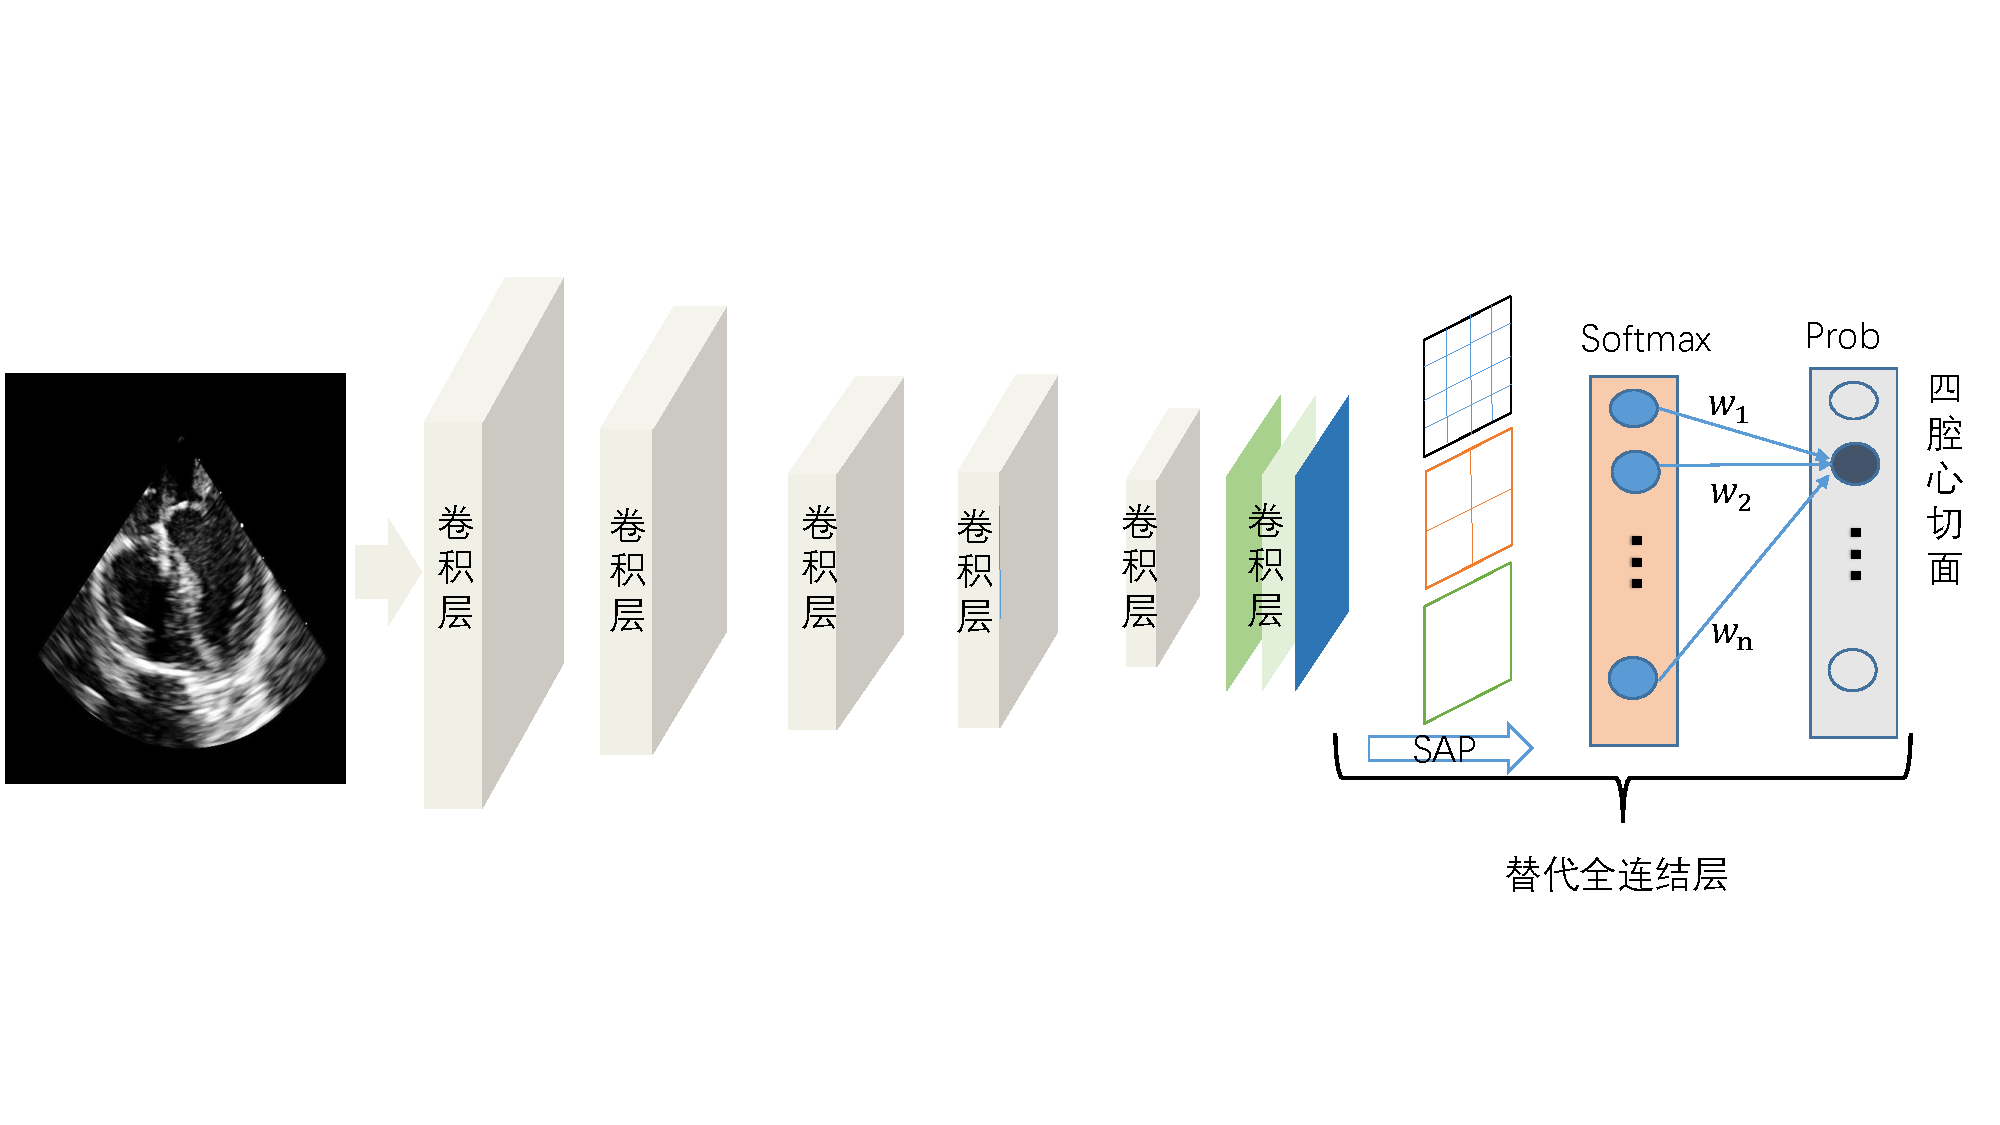
\includegraphics[trim = 30mm 0mm 30mm 0mm, clip, width=0.45\textwidth]{ch03_02}
    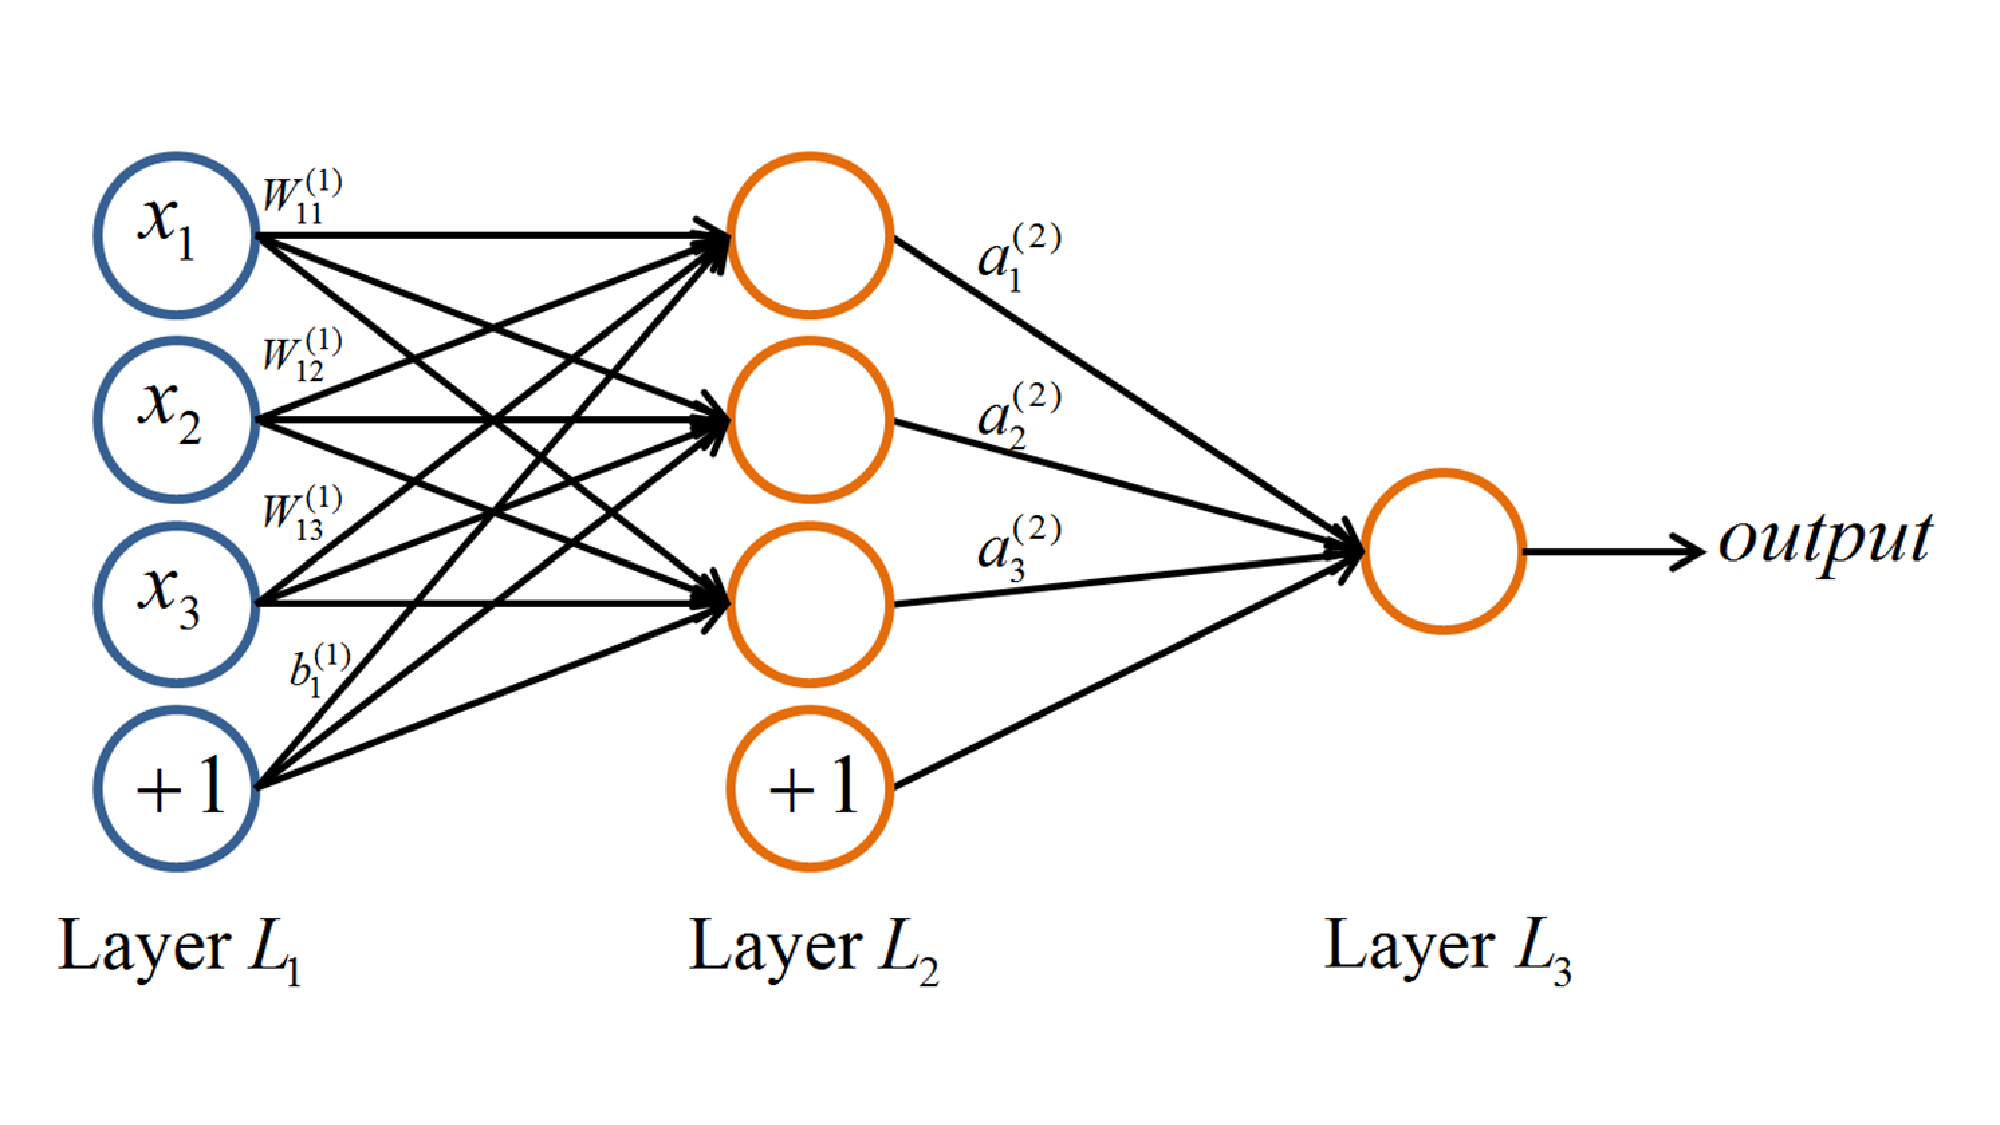
\includegraphics[width=0.9\textwidth]{ch02_01}
    \caption{前馈神经网络(也称为多层感知器)结构示例示意图}
    \label{fig:ch02_01}
\end{figure}

由于神经网络的非线性导致大多数代价函数都变得非凸,需使用迭代的基于梯度的优化,基于极大似然估计的随机梯度下降方法是目前最常用优化的方法,它将参数$\Theta$拟合到训练集 $\mathcal{D}$。反向传播(back propagation)算法可以用来高效地计算复杂函数的梯度,随机梯度下降中一般使用批量数据的一小部分用于梯度更新,在实践中优化最大可能性等价于最小化负对数似然,它与训练数据和模型分布间的交叉熵等价:
\begin{equation}
 \arg \min_{\Theta} - \sum^{N}_{n = 1} \log\big[ P(y_{n}| {\bf x}_{n}; \Theta) \big].
\end{equation}
其通常不直接优化我们感兴趣的目标,例如ROC曲线下的面积或用于分割的常用评估度量(例如Dice系数),该损失也称为交叉熵代价损失,。

长期以来,深度神经网络(Deep Neural Network,DNN)随着层数加深,优化函数越来越容易陷入局部最优解导致梯度弥散问题难以有效训练。从2006年开始才重新受到欢迎\citep{Hinton2006a},指出两种流行的无监督网络结构:堆叠自动编码器和深度置信网络,可以以无监督的方式逐层训练(预训练)DNN。但这些技术相当复杂需要大量手动调参才能产生令人满意的效果。

目前,最流行的模型是以有监督的方式进行端对端训练,通过引入预处理和新的激活函数,极大地简化了训练过程。最流行的网络结构是卷积神经网络和递归神经网络。尽管递归神经网络越来越受欢迎,但CNN目前在(医学)图像分析中应用最广泛。以下各节将简要介绍这些方法,从最受欢迎的方法开始,并讨论它们在应用于医疗问题时的差异和潜在的挑战。

\subsection{卷积神经网络}

卷积神经网络(CNN)是多层前馈神经网络的一种特例,是一种专门用来处理具有类似网格结构的数据的神经网络。,例如时间序列数据(可以认为是在时间轴上有规律地采样形成的一维网格)和图像数据(可以看作是二维的像素网格)。较普通神经网络引入了感受野、卷积核滤波器组、卷积层、池化层等概念,其隐藏层的神经元设计成跟上一层神经元局部稀疏连接,并利用参数共享来减少模型复杂度。针对图像这种结构化数据,由不同卷积核来探测不同空间位置上的局部统计特征。通过堆叠多层的卷积结构,实现从低层到高层语义空间的抽象映射。
\begin{figure}[!htbp]
    \centering
    %trim option's parameter order: left bottom right top
    %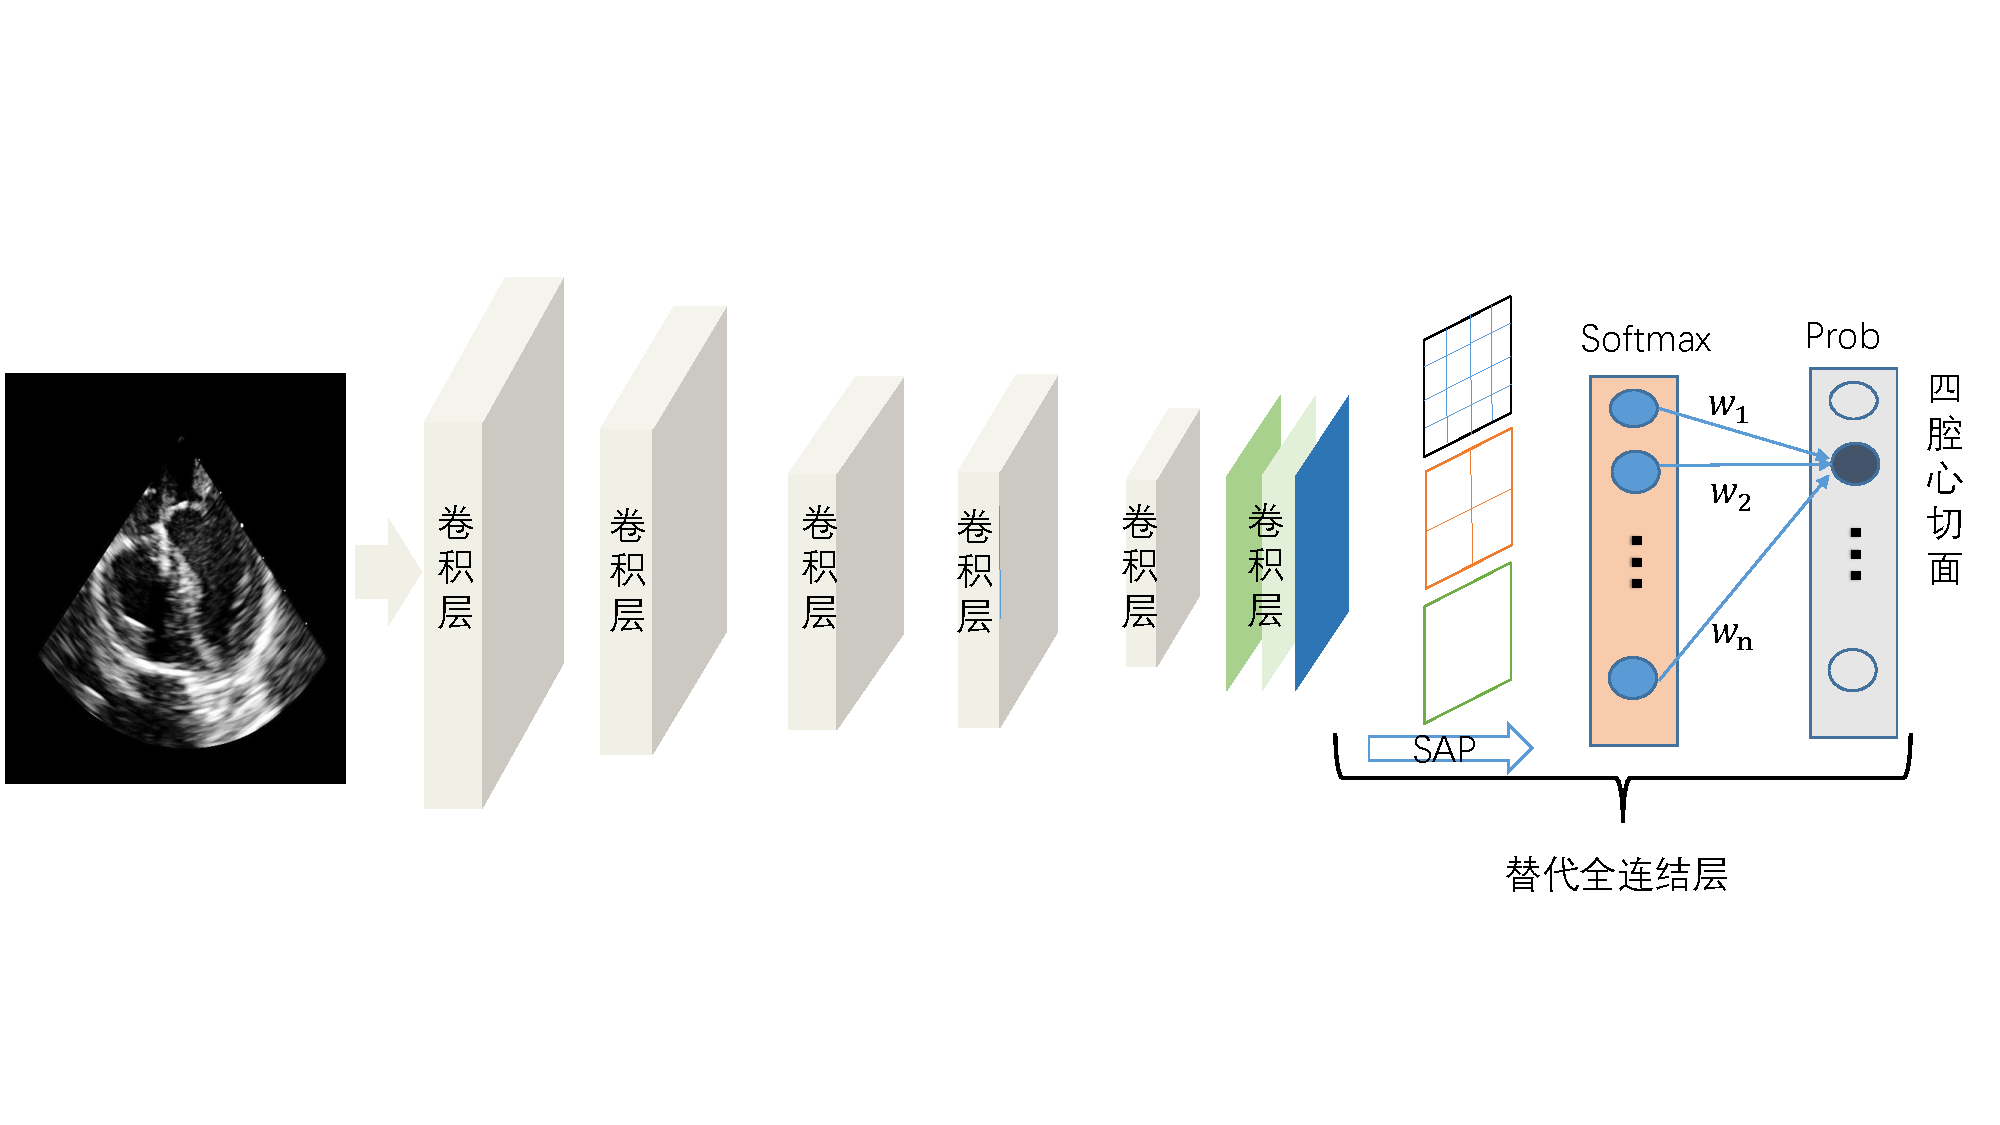
\includegraphics[trim = 30mm 0mm 30mm 0mm, clip, width=0.45\textwidth]{ch03_02}
    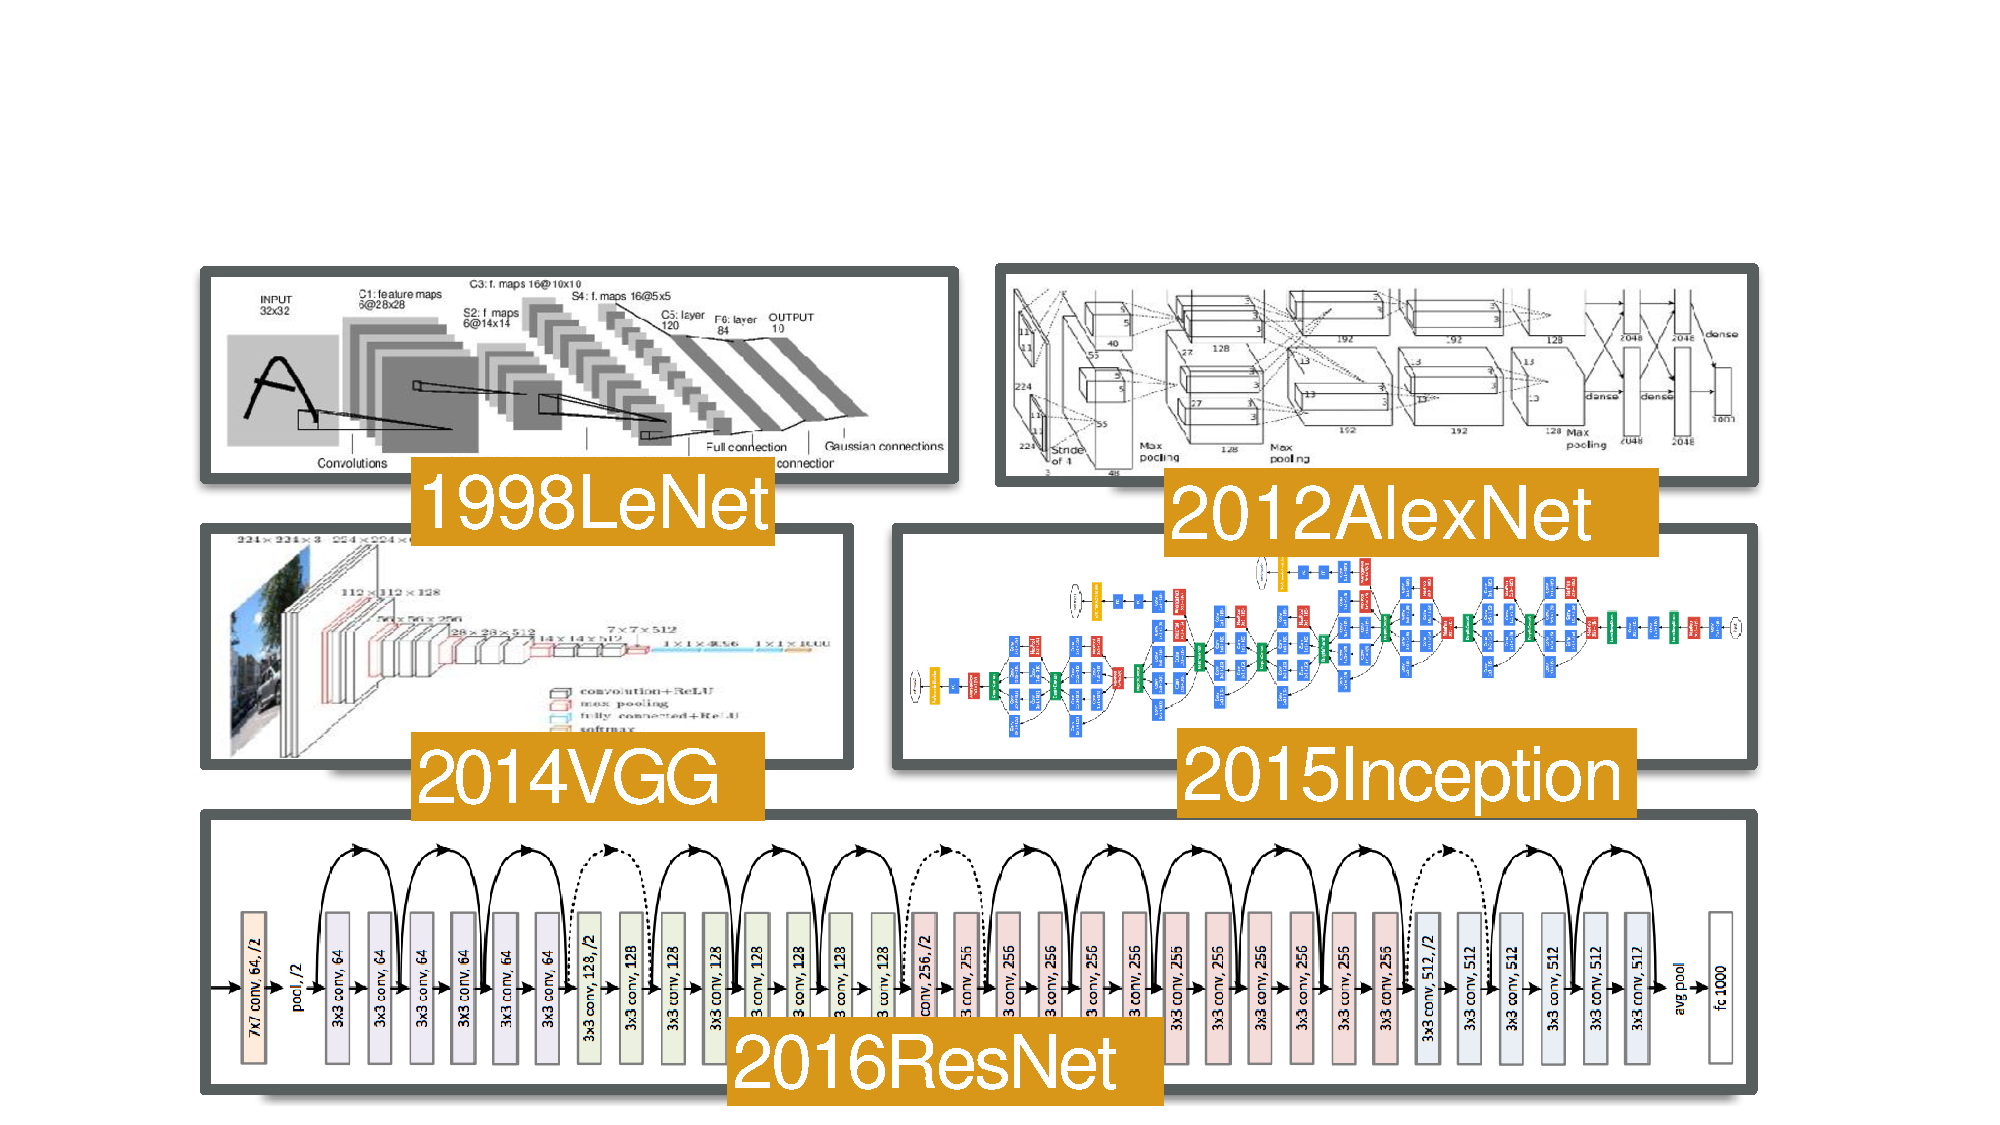
\includegraphics[width=0.9\textwidth]{ch02_02}
    \caption{经典深度网络结构示意图}
    \label{fig:ch02_02}
\end{figure}
MLP和CNN之间有两个关键的区别:首先,网络中的权重以网络对图像执行卷积操作的方式共享。这样,模型不需要为在图像中不同位置出现的同一对象分别检测单独的检测器,从而使网络在输入的平移时保持不变性。它还大大减少了需要学习的参数数量(即权重的数量不再取决于输入图像的大小)。图\ref{fig:ch02_02}中显示了LeNet-5\citep{Jarrett2009}的经典网络结构。

在每一层,输入图像与一组$K$卷积核进行卷积: $\mathcal{W} = \{ {\bf W}_{1}, {\bf W}_{2}, \ldots, {\bf W}_{K} \}$ 并添加偏差项$\mathcal{B} = \{b_{1}, \ldots, b_{K}\}$,每个生成一个新的特征映射(feature map)${\bf X}_{k}$。这些特征受到非线性变换$\sigma(\cdot)$的影响,并且对每个卷积层$l$重复相同的过程:
\begin{equation}
\label{eq::mapping_cnn}
 {\bf X}_{k}^{l} = \sigma\big( {\bf W}_{k}^{l -1} \ast {\bf X}^{l -1} + b_{k}^{l-1} \big).
\end{equation}

其次,在于CNN中的池化层(Pooling),其中邻域的像素值使用置换不变函数(通常是最大或平均运算)进行聚合。这会导致一定量的平移不变性,并再次减少网络中的参数数量。在网络的卷积层结束时,通常会添加全连接的层(即常规的神经网络层),其不再共享权重。类似于MLP,通过softmax函数概率归一化提供最后输出层中的激活值,并且使用方向传播优化极大似然损失对网络进行训练,从而产生类别概率分布。
\section{深度卷积神经网络}
鉴于CNN在医学图像分析中的流行,将详细介绍广泛使用的模型中最常见的网络结构及其差异,相关的方向的演进请参考图\ref{fig:ch02_04}。
\begin{figure}[!htbp]
    \centering
    %trim option's parameter order: left bottom right top
    %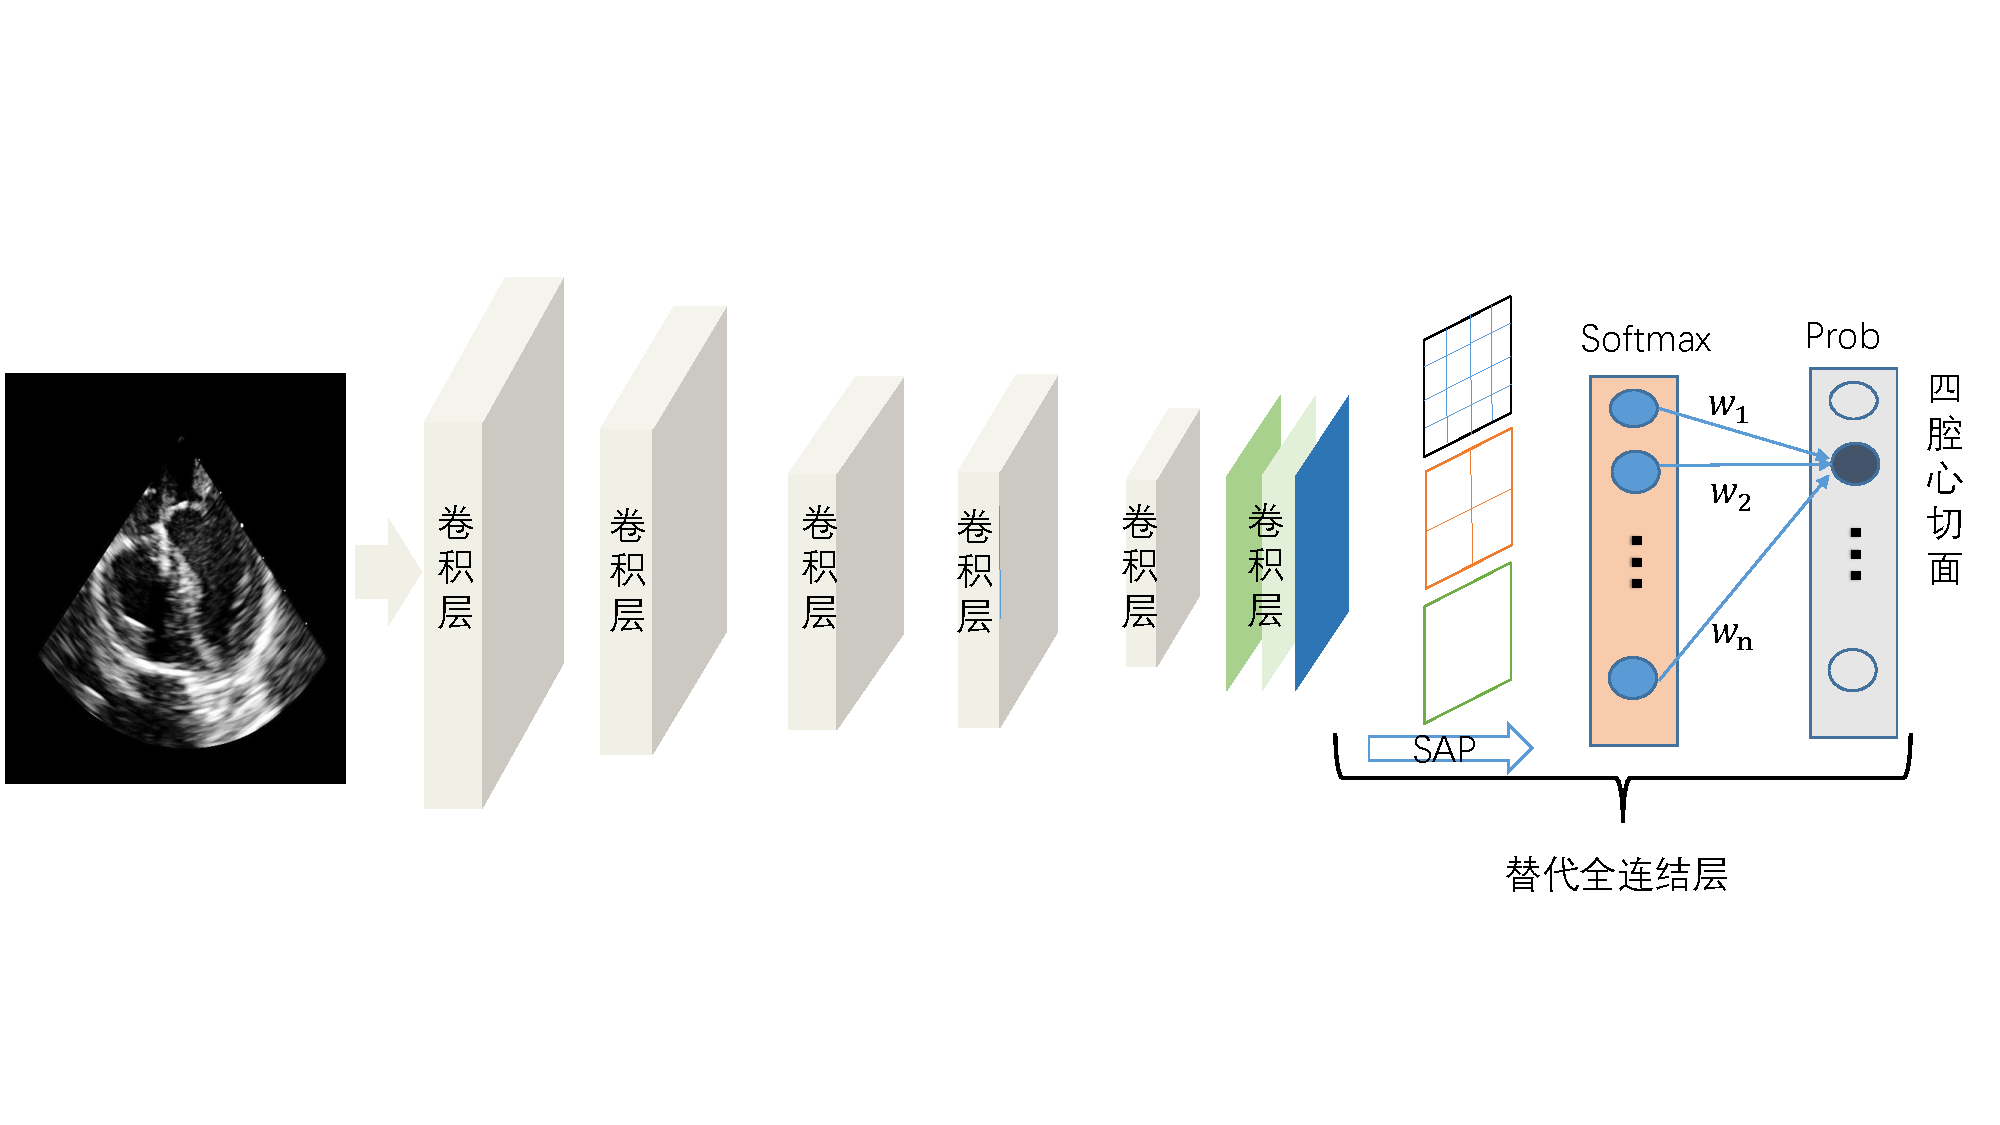
\includegraphics[trim = 30mm 0mm 30mm 0mm, clip, width=0.45\textwidth]{ch03_02}
    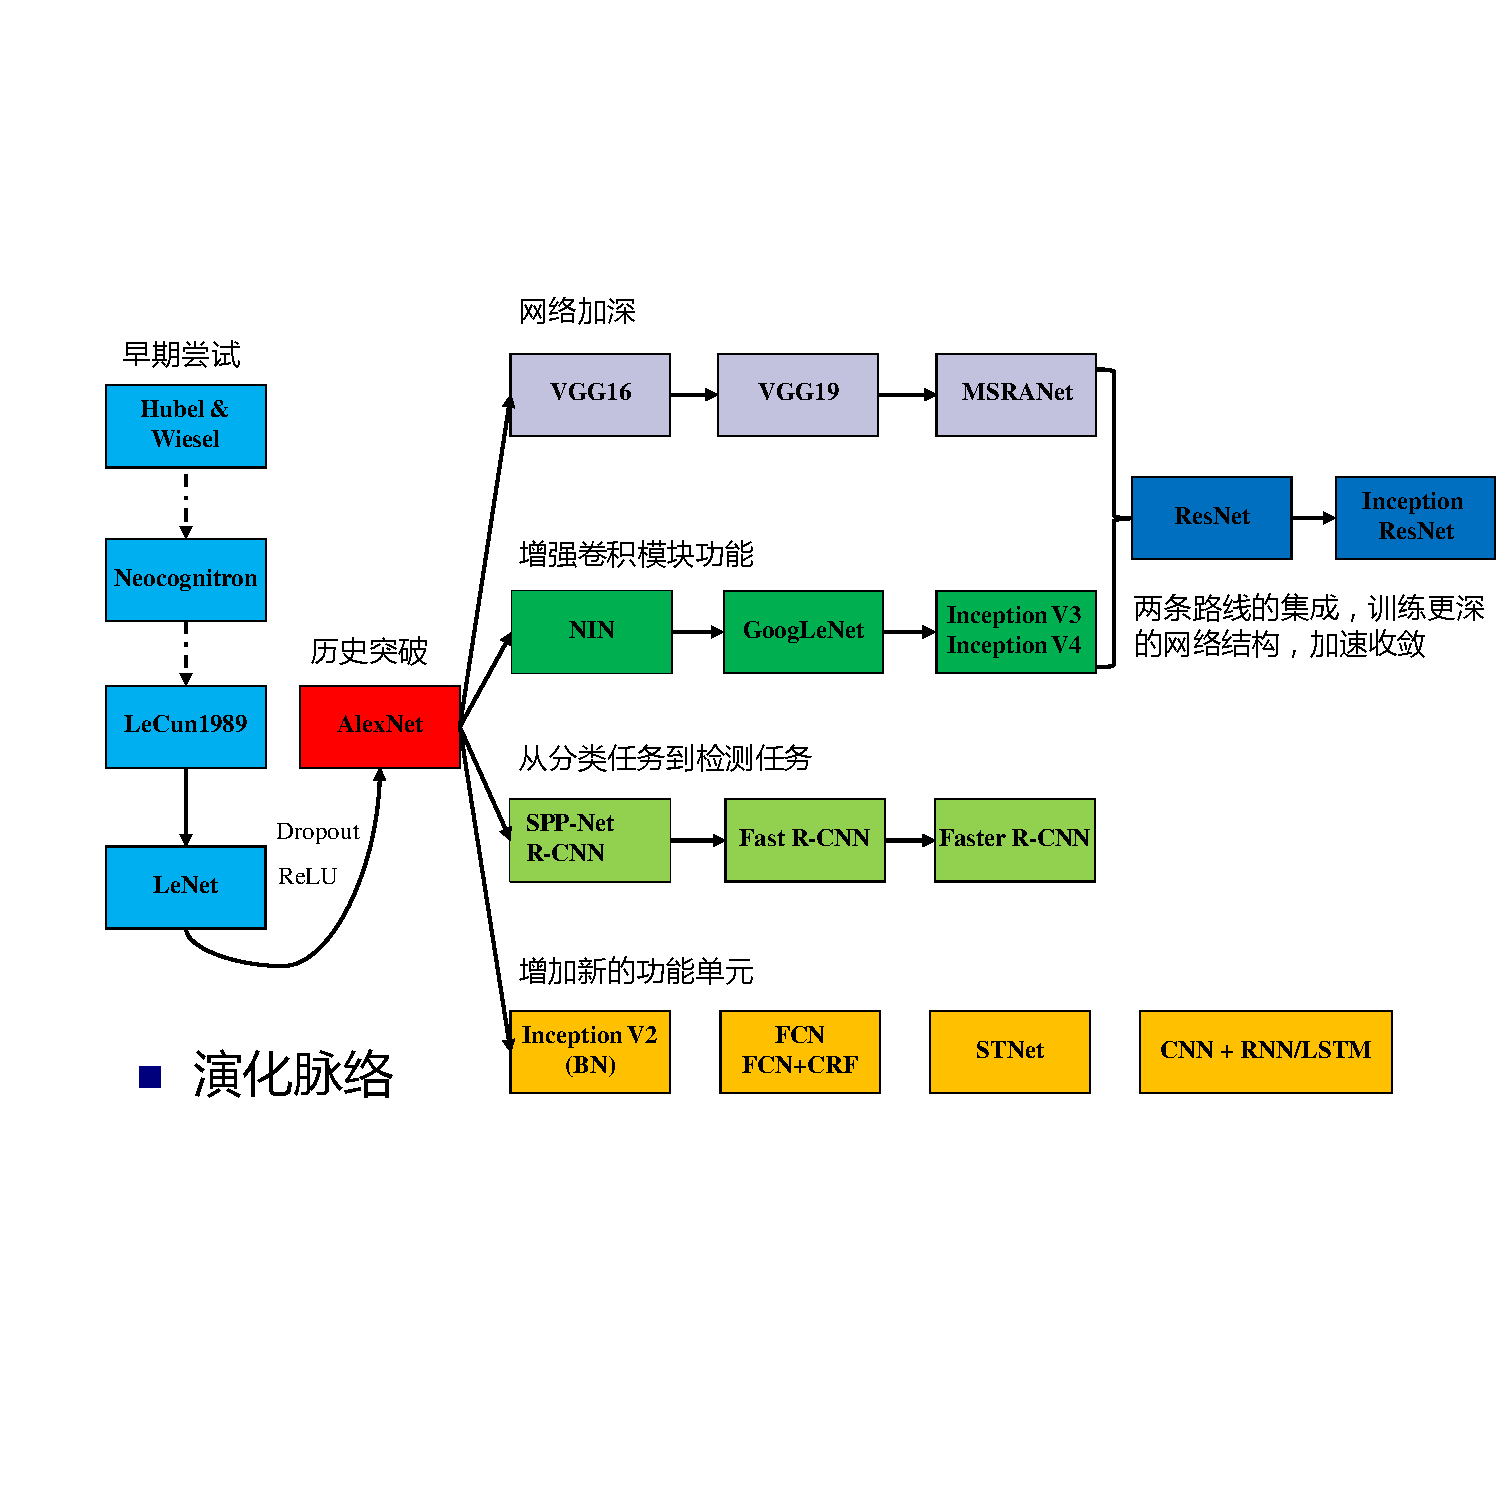
\includegraphics[height=60mm,width=0.9\textwidth]{ch02_04}
    \caption{深度卷积神经网络结构演进图}
    \label{fig:ch02_04}
\end{figure}
 
\subsection{通用分类框架}

深度CNN的典型结构AlexNet\cite{Krizhevsky2012}是在{\it LeNet}模型\citep{Jarrett2009}的基础上引入修正线性单元(Rectified Linear Units,ReLU)的激活函数和Dropout等技术\citep{Krizhevsky2012}进行的改进。模型的激活函数没有采用Sigmoid函数或双曲正切函数,而是选择ReLU函数,目的是引入更多非线性来加速训练收敛速度,解决多层网络反向传播中梯度弥散的问题。为了使得每层输入的分布更平稳,一般引入批量归一化层(Batch Normalization,BN)\cite{Ioffe2014Batch},采用最大池化层进行下采样,有时也把“卷积-激活-归一化-池化”统称为卷积层。最后需连接全连接层,全连接层就不再保存空间信息,是对低层特征的高层抽象,最终输出指定维度大小的向量,作为该图像的特征向量送入最终的分类器进行分类评估。
\begin{figure}[!htbp]
    \centering
    %trim option's parameter order: left bottom right top
    %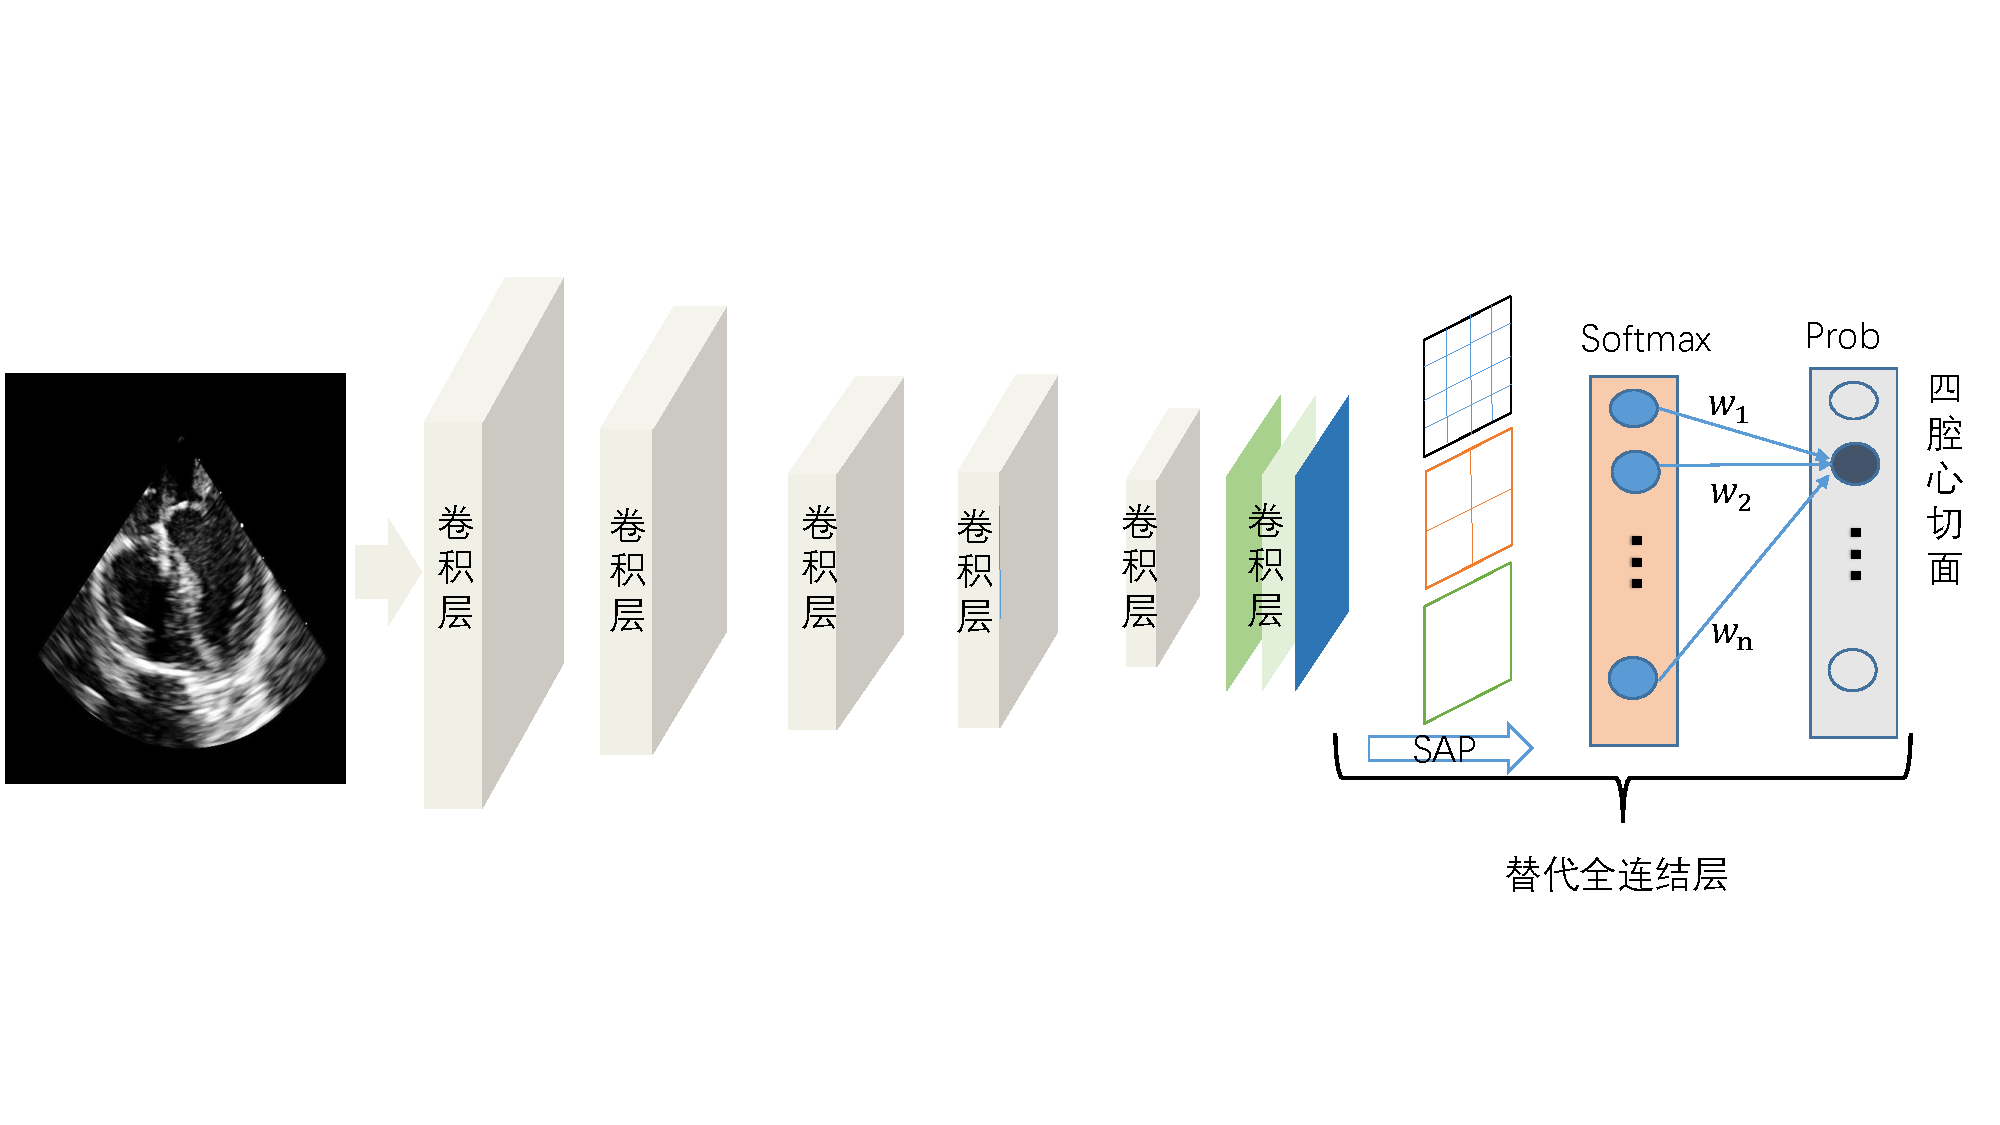
\includegraphics[trim = 30mm 0mm 30mm 0mm, clip, width=0.45\textwidth]{ch03_02}
    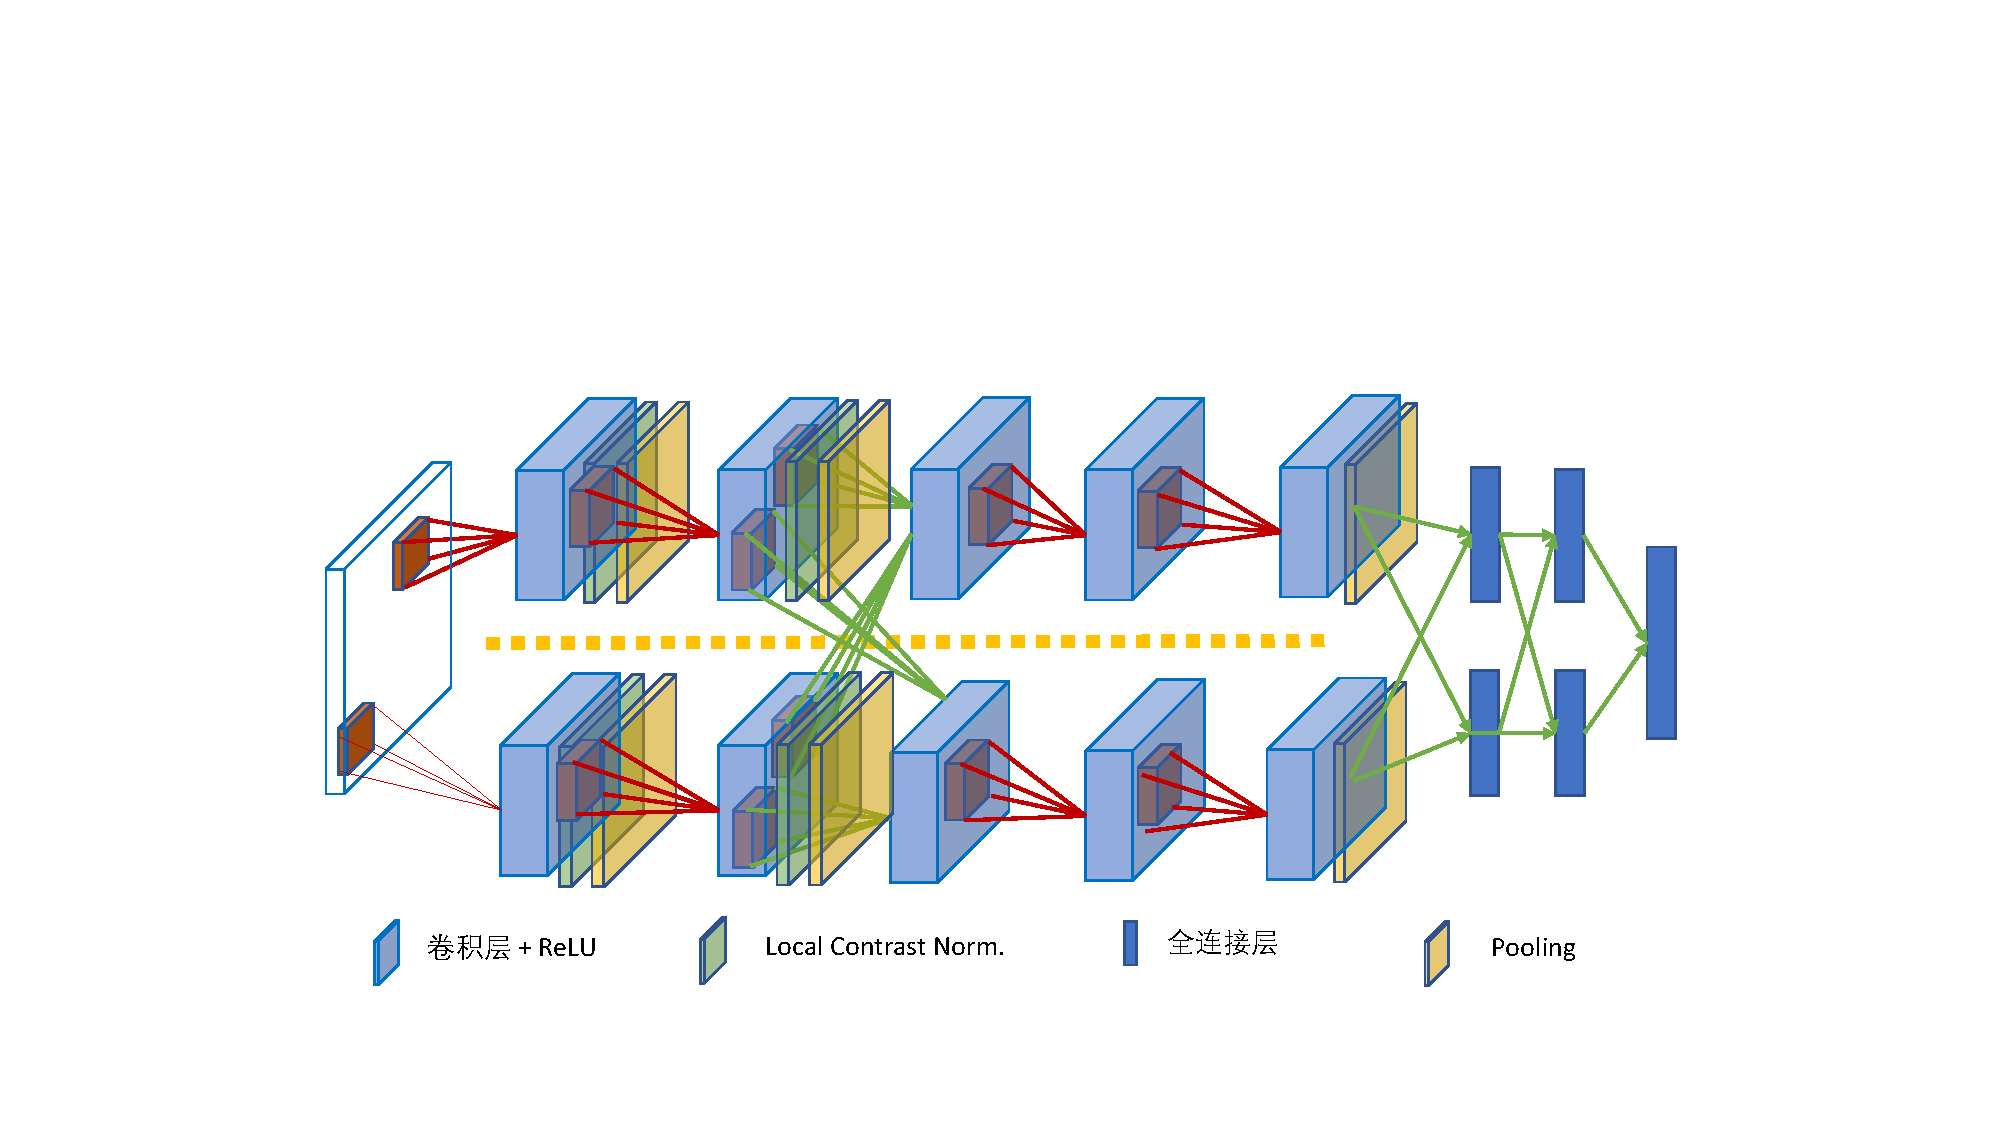
\includegraphics[width=0.9\textwidth]{ch02_03}
    \caption{AlexNet网络结构示意图\cite{Krizhevsky2012}}
    \label{fig:ch02_03}
\end{figure}
2012年以来新的网络结构不断涌现,模型更倾向于更深更复杂的结构。堆叠更小尺寸的卷积核,可以用较少的参数来表示类似的函数,这些更深的网络结构在推断时通常具有较低的内存占用量,这使得它们能够部署在诸如智能手机的移动计算设备上。{\it VGG}\citep{Simonyan2014a}是第一个探索更深层次的网络,网络的结构非常一致,从头到尾全部使用的是$3 \times 3$的卷积和$2\times 2$的池化层。Szegedy等\cite{Szegedy2015}提出了一个名为{\it GoogLeNet}的22层网络,在深层网络之上,引入了更复杂的构建模块,它使用使用密集连接结构用于估计稀疏CNN,也称为{\it Inception}模块\citep{Lin2013a},该模块使用一组不同大小的卷积$1 \times 1,3 \times 3,5 \times 5$的卷积取代了公式\eqref{eq::mapping_cnn};同时把顶部使用的全连接层替换成平均池化层,可以提高训练过程的效率,并再次减少参数的数量。{\it ResNet}网络结构\citep{he15}赢得了2015年的ImageNet挑战,其引入跳跃连接,残差块不是直接学习函数,而是仅学习残差,并因此预先调整每一层中学习接近同等函数映射,这样可以有效地训练更深的网络模型,可以认为{\it ResNet}是不同长度的网络的指数集合。

自2017年以来,ImageNet基准测试的性能已经饱和\cite{Deng2009ImageNet},虽然仍有很多分类识别的工作进行网络结构的设计,但很难评估性能的小幅增长是否真的归因于“更好”和更复杂的架构。这些模型所提供的较低内存占用空间的优势通常对于医疗应用来说并不重要。因此,{\it AlexNet}或其他简单模型(如{\it VGG、ResNet})仍然很受医学数据分析领域欢迎。

\subsection{多通路的卷积神经网络结构}
\label{sec:mc_architectures}
将深度学习技术应用于医疗领域的挑战通常在于将现有网络结构适应于例如不同输入格式,例如三维数据。在CNN早期应用于这样的体积数据时,通过将感兴趣体积(VOI)划分为切片,将全部3D卷积和由此产生的大量参数分开,所述切片作为不同的流馈送到网络。文献\citepns{Prasoon2013Deep}是第一个将这种方法用于膝关节软骨分割的。类似地,网络可以以多通道方式从3D空间中馈入多个角度的贴片\citep{Roth2014A},这些方法也被称为2.5D分类。

根据不同任务需要、不同融合方式可以得出多通路的网络结构,多个输入CNN网络的特征图可以在网络的任何处合并融合。如双通道架构\cite{Kamnitsas2017}可应用于多尺度图像分析;
在图像检测任务中,为了检测指定对象区域,上下文往往是一个重要的提示,增加上下文最直接的方法是将更大的区域块提供给网络,但这会显著增加网络的参数和内存需求量。因此除了提高分辨率获得局部信息之外,还可引入多通道多尺度网络结构\cite{Farabet2013Learning},一些医学应用也成功地使用该概念\citep{Kamnitsas2017,Moeskops2016Automatic,Song2015Accurate,Yang2016Cascade}。

\subsection{全卷积网络结构}
\label{sec:fully_arch}

分割和去躁是自然和医学图像分析中的一项常见任务,为了解决这个问题,CNN可分别对图像中的每个像素进行分类,需要在特定像素周围提取区域块。该“滑动窗口”方法的缺点是来自相邻像素的输入块具有巨大的重叠并且多次计算相同的卷积操作,卷积和点积都是线性算子,因此内积可以写成卷积,反之亦然,通过将全连接的层重写为卷积,CNN可以输入大于其被训练的图像尺寸的任意图像,并生成概率图。但由于池化合并图层,这可能导致输出的分辨率远远低于输入,反卷积\citep{Long2017Fully}是为防止这种分辨率下降而提出上采样方法之一,如图\ref{fig:ch02_05}。通过将结果拼接在一起,减去由于“有效”卷积而丢失的像素,可以获得最终输出的全分辨率完整输出。
\begin{figure}[!htbp]
    \centering
    \begin{subfigure}[b]{0.45\textwidth}
        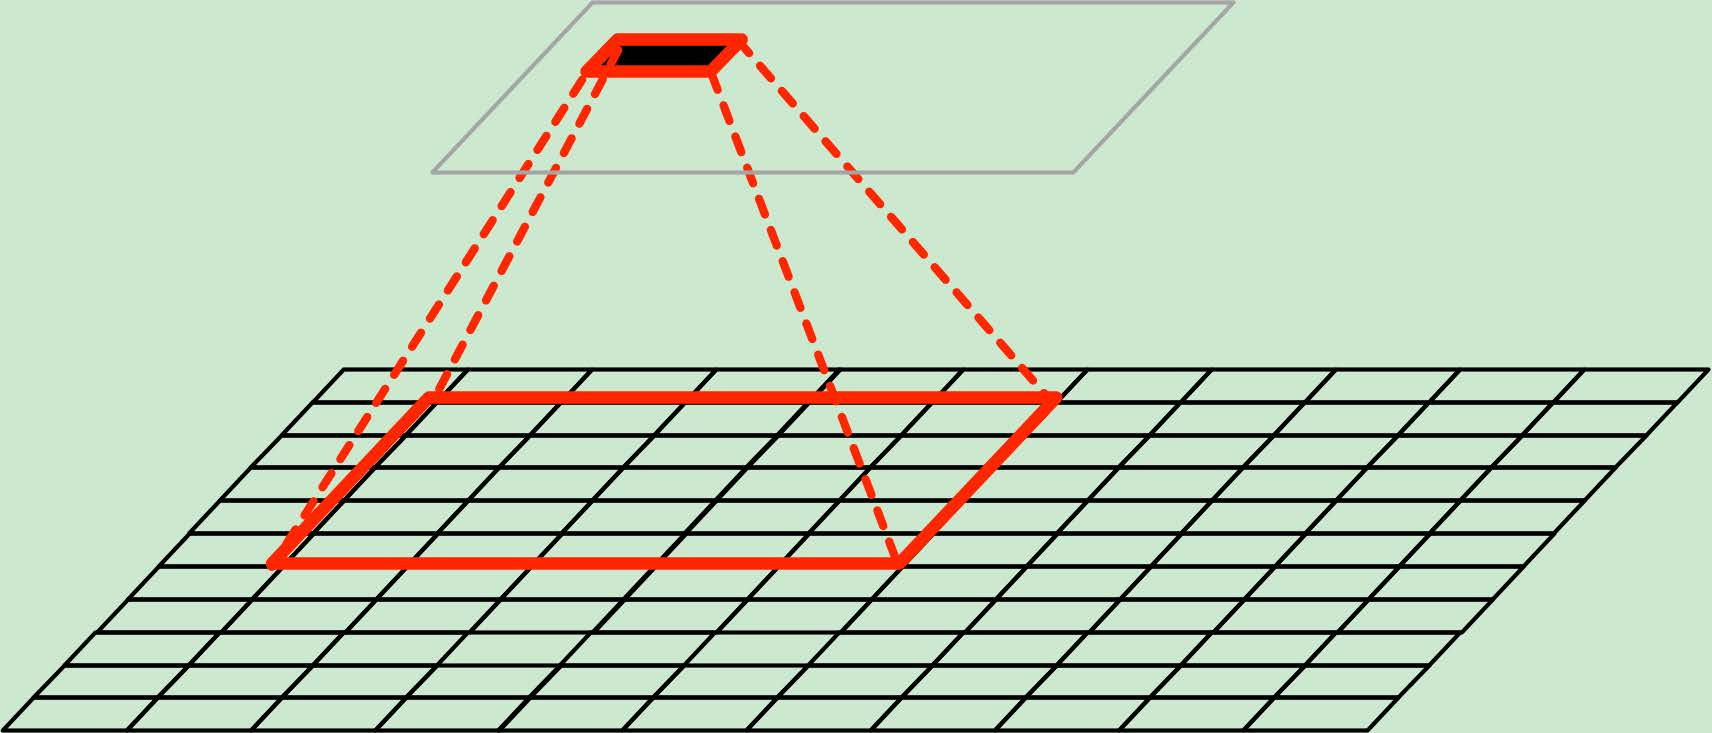
\includegraphics[height=30mm,width=\textwidth]{ch02_05_1}
        \caption{卷积}
        \label{fig:ch02_05_1}
    \end{subfigure}%
    % add desired spacing
    \begin{subfigure}[b]{0.45\textwidth}
        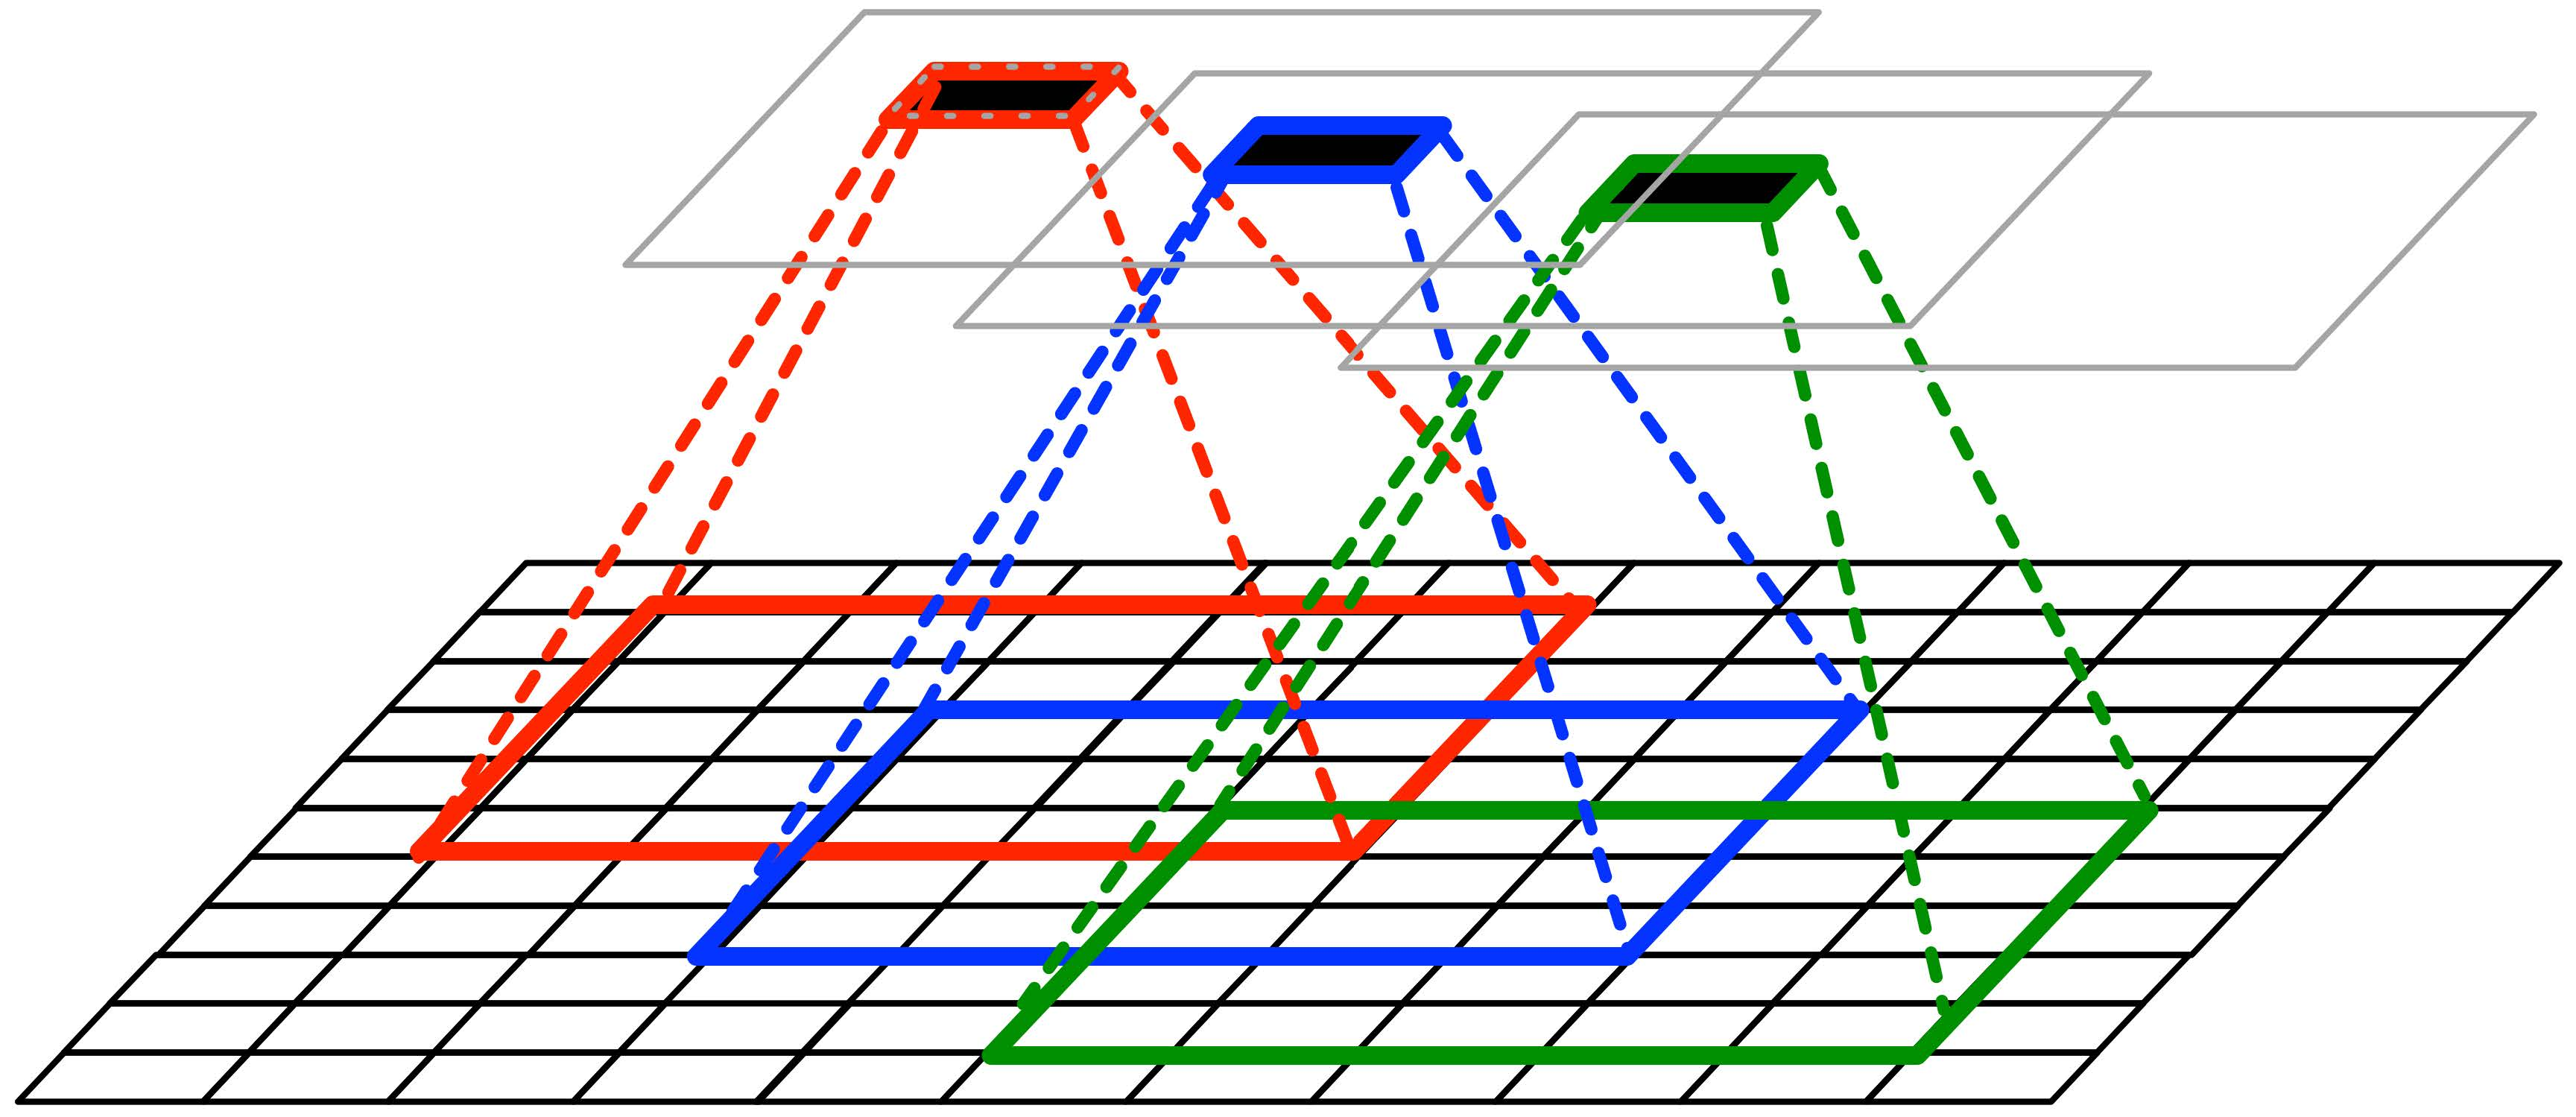
\includegraphics[height=30mm,width=\textwidth]{ch02_05_2}
        \caption{平铺卷积}
        \label{fig:ch02_05_02}
    \end{subfigure}
    % add desired spacing
    \begin{subfigure}[b]{0.45\textwidth}
        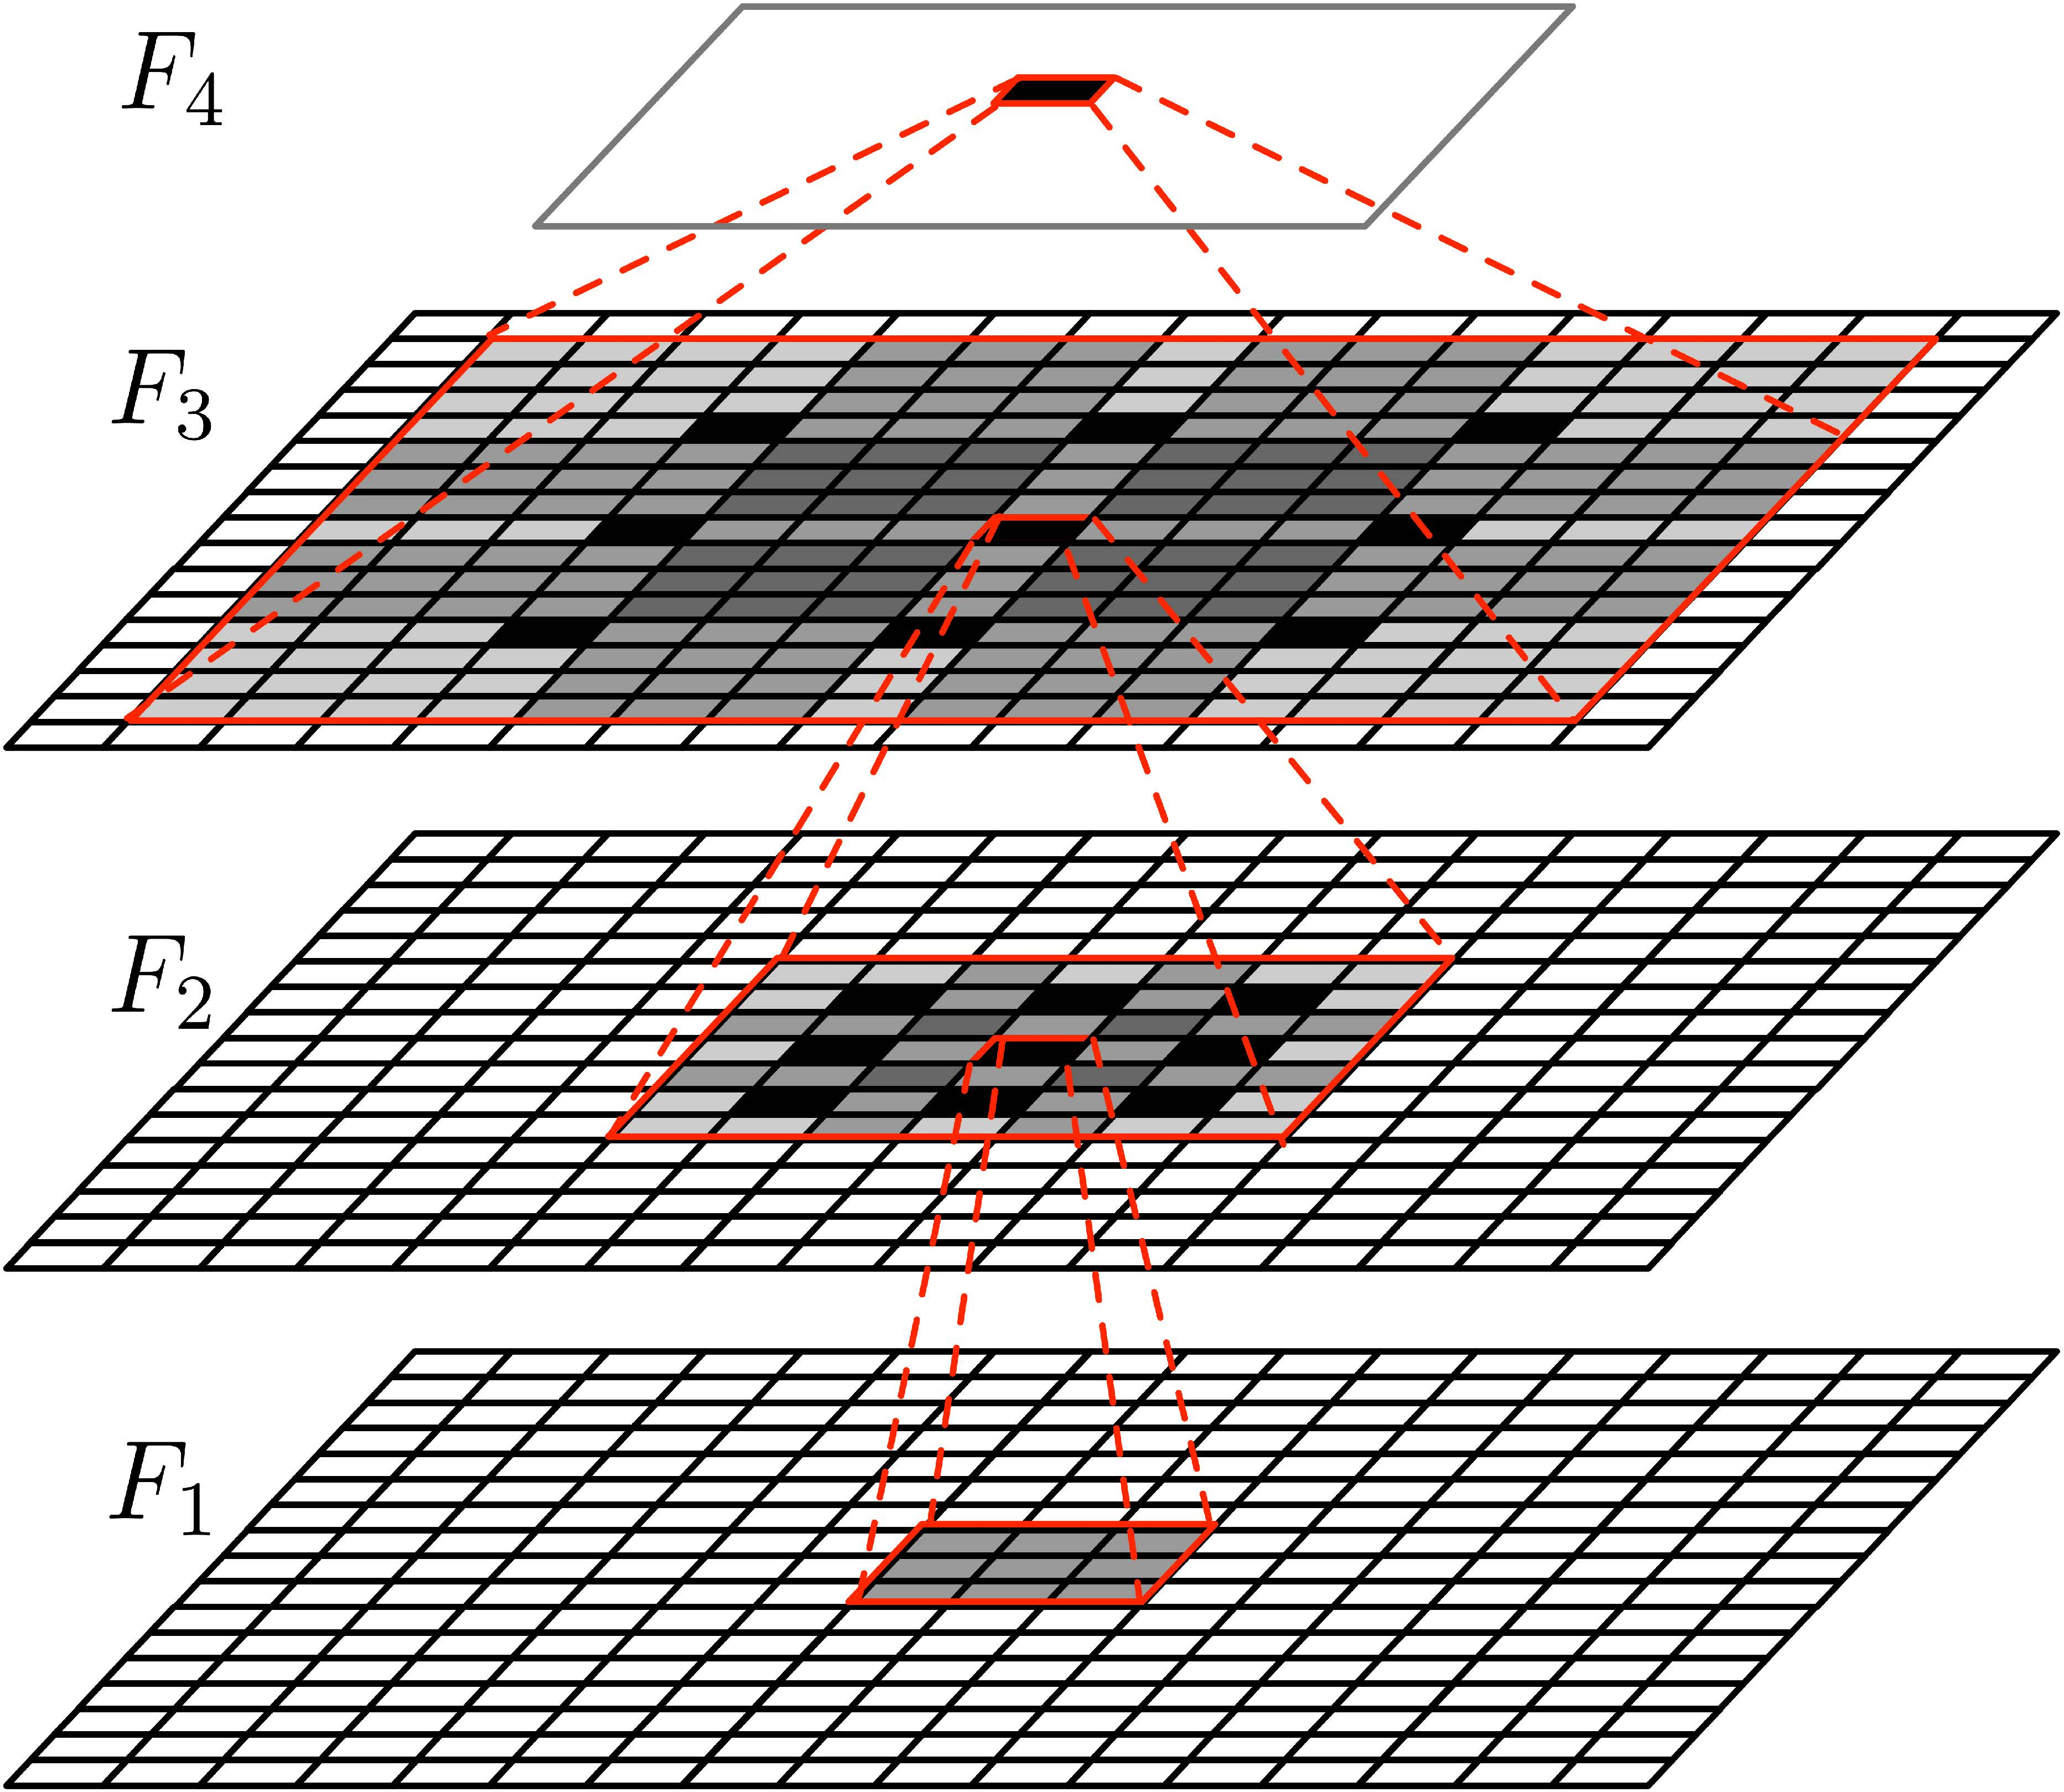
\includegraphics[height=30mm,width=\textwidth]{ch02_05_3}
        \caption{扩张(dilated)卷积}
        \label{fig:ch02_05_03}
    \end{subfigure}
    % add desired spacing
    \begin{subfigure}[b]{0.45\textwidth}
        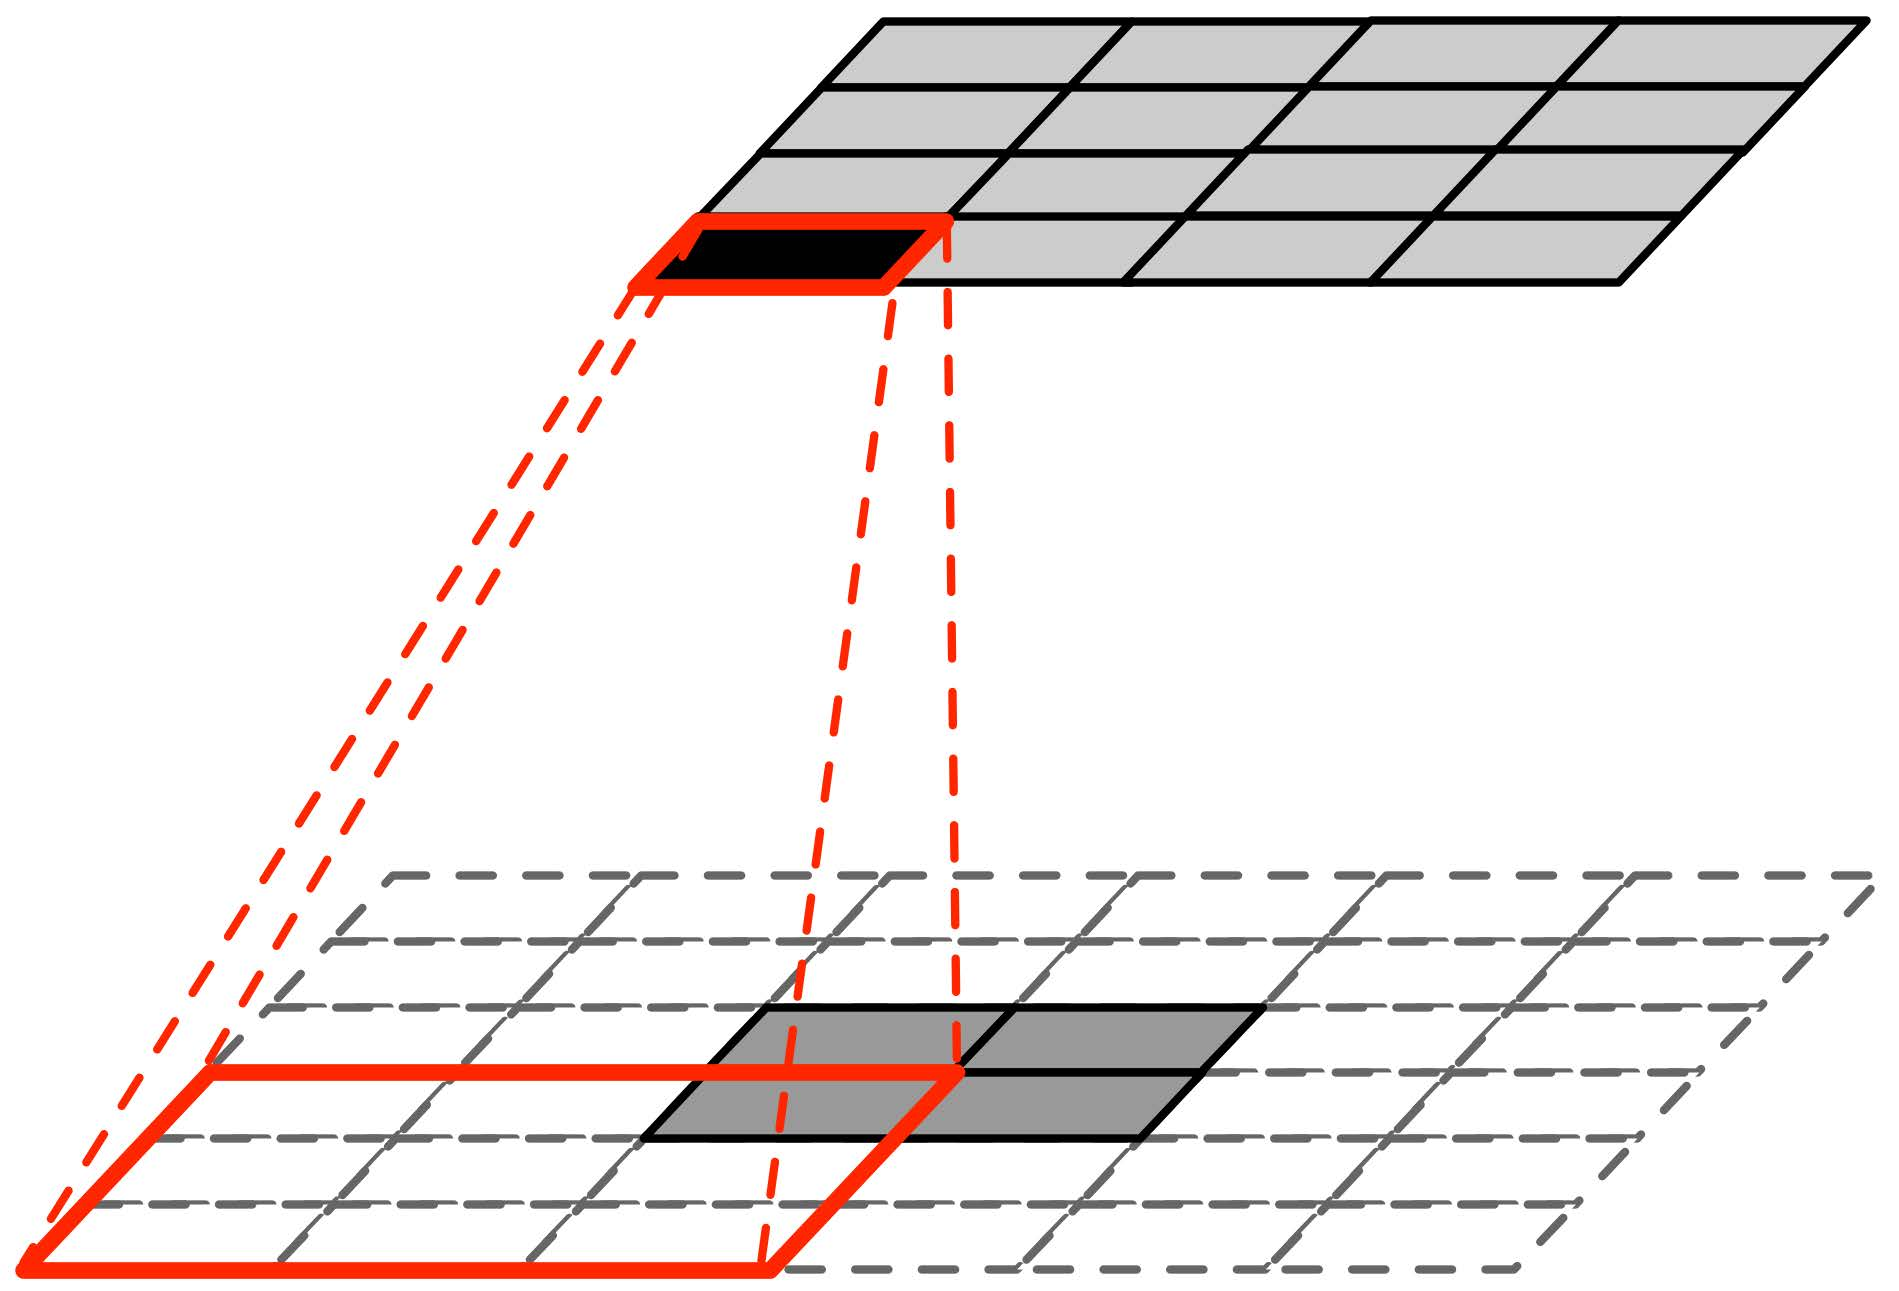
\includegraphics[height=30mm,width=\textwidth]{ch02_05_4}
        \caption{反卷积}
        \label{fig:ch02_05_04}
    \end{subfigure}
    \caption{卷积网络中的各种卷积操作图}
    \label{fig:ch02_05}
\end{figure}
将全卷积网络进一步改进提出U-net架构\cite{Ronneberger2015},其包含一个常规的全卷积结构,后面跟着一个上采样部分,其中反卷积用于增加图像大小,通过收缩编码-膨胀解码(Encoder-Decoder),将它与跳跃连接\citep{he15}相结合,提出Encoder-Decoder卷积层。3D数据也适用类似的方法,如用于体数据的V-Net结构,提出包含类似ResNet的残余块和随机丢失(Drop)层,损失函数也不是传统的交叉熵,而是直接最小化常用的分割误差测量损失\cite{Milletari2016}。

\section{循环神经网络}
\label{sec:rnns}

传统上RNN是为处理序列数据而开发的,可以看作是MLP的泛化,输入和输出的长度都不相同,这使得它们适用于诸如机器翻译、语音识别这样的任务,其中源语言和目标语言的句子是输入和输出。在分类设置中,模型学习了给出一个可变长度序列${\bf x}_{1}, {\bf x}_{2}, \ldots, {\bf x}_{T}$的类别$P(y | {\bf x}_{1}, {\bf x}_{2}, \ldots, {\bf x}_{T}; \Theta)$,而不是一个输入向量${\bf x}$。

普通的RNN在$t$时刻维持一个隐式或隐藏状态${\bf h} $,它是从其输入${\bf x}_{t}$和前一状态${\bf h}_{t-1}$:
\begin{equation}
 {\bf h}_{t} = \sigma({\bf W}{\bf x}_{t} + {\bf R}{\bf h}_{t - 1} + {\bf b}),
\end{equation}

其中加权矩阵${\bf W}$和${\bf R}$是随时间共享的。对于分类,通常会添加一个或多个完全连接的层,然后添加softmax以将序列映射到类别概率: 
\begin{equation}
 P(y | {\bf x}_{1}, {\bf x}_{2}, \ldots, {\bf x}_{T}; \Theta) = \text{softmax}( {\bf h}_{T}; {\bf W}_{out}, {\bf b}_{out}).
\end{equation}

由于梯度需要通过时间从输出反向传播,因此RNN具有固有的深度(及时性),因此与常规深层神经网络一样遭受梯度弥散难以训练问题。为此已经设计几种专用单元来解决上下文依赖问题,最早和最流行的是长期短期记忆(Long Short-Term Memory,LSTM)单元\citep{Hochreiter1997Long},而门控复发单元(Gated Recurrent Unit,GRU)\citep{Cho2014Learning}是LSTM的最新简化版。

尽管最初提出是针对一维输入,但RNN越来越多地应用于图像,在自然图像中,“pixelRNN”被用作自回归模型,生成模型最终可以生成类似于训练集样本的新图像。对于医疗应用,它们已被用于分割问题,并且在各种竞赛挑战中得到令人鼓舞的结果\citep{Stollenga2015Parallel}。

\section{无监督深度学习}
\subsection{自编码器}
自编码器(Auto-encoders,AE)是简单神经网络的一种,通过一个隐藏层${\bf h}$来产生编码(code)${\bf x}'$近似表示输入${\bf x}$。重建其隐藏层${\bf W}_{h, x'}$ 和相应的偏差$b_{h, x'}$,它们由权重矩阵和输入到隐藏状态和${\bf W}_{x, h}$的偏置$b_{x, h}$来控制。非线性函数用于计算隐藏激活: 
\begin{equation}
\label{eq::ae_projection}
 {\bf h} = \sigma({\bf W}_{x, h} {\bf x} + {\bf b}_{x, h}).
\end{equation}
此外,隐藏层$|{\bf h}|$的维度小于$|{\bf x}|$。这样,数据被投影到表示输入中的主要潜在结构的较低维子空间上。如果隐藏层的大小与输入大小相同,并且不再添加非线性,则模型将简单地学习标识函数,正则化或稀疏性约束可以用来增强发现过程。

去噪自动编码器\citep{Vincent2010Stacked}是另一种防止模型学习微不足道解决方案的解决方案。这里模型被训练来重构来自噪声损坏版本(通常是盐和胡椒噪声)的输入。SAE(或深度AE)通过将自动编码器层放置在彼此之上而形成。相关医疗应用中,自动编码器层经常被(“贪婪算法”)单独训练,然后使用监督训练对整个网络进行微调以进行预测。

\subsection{受限波兹曼机和深度信念网络}
受限玻尔兹曼机(Restricted Boltzmann Machines,RBMs)\citep{Hinton2006a}是一种马尔可夫随机场,构成输入层或可见层${\bf x} = (x_{1}, x_{2}, \ldots, x_{N})$和一个带有潜在特征表示的隐藏层${\bf h} = (h_{1}, h_{2}, \ldots, h_{M})$。节点之间的连接是双向的,因此给定输入向量$\bf x$可以获得潜在特征表示$\bf h$,反之亦然。因此,RBM是一个生成模型,我们可以从中进行抽样并生成新的数据点。与物理系统类比,能量函数被定义为输入和隐藏单位的特定状态$({\bf x}, {\bf h})$:
\begin{equation}
 E({\bf x}, {\bf h}) = {\bf h}^{T}{\bf W}{\bf x} - {\bf c}^{T}{\bf x} - {\bf b}^{T}{\bf h},
\end{equation}
与 ${\bf c}$ and ${\bf b}$ 偏差条款。系统的“状态”的概率通过将能量传递给指数和正态化来定义:
\begin{equation}
 p({\bf x}, {\bf h}) = \frac{1}{Z} \exp\{ - E({\bf x}, {\bf h}) \}.
\end{equation}
计算分区函数 $Z$通常是棘手的。然而,以${\bf h}$为条件计算${\bf v}$形式的条件推断是可以处理的,并且会产生一个简单的公式:
\begin{equation}
 P(h_{j} | {\bf x}) = \frac{1}{ 1 + \exp\{ -b_{j} - {\bf W}_{j}{\bf x}\} }.
\end{equation}
由于网络是对称的,类似的表达式适用 $P(x_{i} | {\bf h})$.

DBNs \citep{Hinton2009Deep}实质上是AE层被RBM取代的堆叠多层AE。再次,以无人监督的方式进行单个层次的训练。通过向DBN顶层添加线性分类器并执行监督优化来执行最终的微调。
\subsection{变分自编码器和深度生成对抗网络}
最近,引入了两种新颖的无监督网络结构:变分自动编码器(VAE)\citep{Kingma2013Auto}和生成对抗网络(GAN)\citep{Goodfellow2014Generative}。因很难解决它们配分函数的数值而成为众所周知的难题,目前还没发现将这些方法应用于医学图像,但在自然图像中的应用还是值得期待的。

\section{深度学习相关技术}
在本节中,我们将从激活函数,损失函数,正则化和优化四个方面描述CNN的主要改进方向。
\subsection{激活函数}
\label{Activationfunctions}
合适选择激活函数能显着提高了CNN对于某个任务的性能。在本节中,我们将介绍CNN中几种激活函数。

\subsubsection{ReLU}

ReLU激活函数定义如下:
\begin{equation}\label{eq:ReLU}
a_{i,j,k}=\max(0,z_{i,j,k})
\end{equation}
其中$ z_{i,j,k} $是位置$ (i,j) $第$k$个通道的输出,ReLU是一个分段饱和线性函数,它将负数部分修剪为零,并保留正数部分(参见\figurename {\ref{fig:ReLU}})。ReLU的取$ \max $操作的计算速度比sigmoid或tanh激活函数快得多,并且它还可以诱导隐藏单元的稀疏性并允许网络获得稀疏表示。
文献表明,甚至在没有预训练的情况下,使用ReLU可以有效地训练深度网络\cite{Krizhevsky2012}。
\subsubsection{带泄漏的ReLU}

ReLU单元的一个潜在缺点是只要单元不激活,它就具有零梯度。基于梯度的优化不会调整它们的权重,这可能会导致最初没有激活的单位以后永不会激活。此外,由于恒定的零梯度,它可能会减慢训练过程。为了缓解这个问题,Mass等\cite{Maas2013}引入了带泄漏(Leaky)的ReLU(LReLU),其定义如下:
\begin{equation}\label{eq:LReLU}
    a_{i,j,k}=\max(0,z_{i,j,k})+\lambda\min(0,z_{i,j,k})
\end{equation}
其中$ \lambda $是$(0,1)$范围内的预定义参数。与ReLU相比, LReLU使得具有负向值而不是将其映射到常量零点,这使得当单元不活动时允许一个小的非零梯度。
\subsubsection{带参数的整流线性单元}

不同于在LReLU中使用预定义的参数,而是在等式(\ref{eq:PReLU})中给出带参数的整流线性单元(PReLU),其自适应学习参数以提高准确性。在数学上,PReLU函数定义为
\begin{equation}\label{eq:PReLU}
    a_{i,j,k}=\max(0,z_{i,j,k})+\lambda_k\min(0,z_{i,j,k})
\end{equation}
其中$ \lambda_k $是第$ k $通道的待学习参数。由于PReLU仅引入极少量的额外参数,例如,额外的参数数量与整个网络的通道数量相同,因此不会出现过度拟合的额外风险,额外的计算成本可以忽略不计。它也可以通过反向传播与其他参数同时训练。

\subsubsection{随机整流线性单元}\label{RReLU_comp}
LReLU的另一个变体是随机整流线性单元(RReLU)\cite{xu2015ecirical},在RReLU中负值部分的参数从均匀分布中随机抽样,然后在测试中使用固定值(参见\figurename {\ref{fig:RReLU}})。形式上RReLU函数定义如下:
\begin{equation}\label{eq:RReLU}
    a^{(n)}_{i,j,k}=\max(0,z^{(n)}_{i,j,k})+\lambda^{(n)}_k\min(0,z^{(n)}_{i,j,k})
\end{equation}
其中$ z^{(n)}_{i,j,k}$是位置$ (i,j) $上第$n$个样例的第$k$个通道的输出, $ \lambda^{(n)}_k $表示其对应的采样参数,$a^{(n)}_{i,j,k}$表示其相应的输出。由于其随机性,它可以减少过度拟合。Xu等\cite{xu2015ecirical}也对标准图像分类任务中的ReLU,LReLU,PReLU和RReLU进行评估,并得出结论:在整流激活单元中加入一个非零斜率用于负值部分,可以持续改善性能。

\subsubsection{指数线性修正单元}
Clevert等\cite{Clevert2015}引入了指数线性单元(Exponential Linear Unit,ELU),它可以更快地学习深度神经网络,并提高分类精度。像ReLU、LReLU、PReLU和RRELU一样,ELU通过将正部分设置为线性变换来避免渐消梯度问题。与同样具有负值部分的LReLU,PReLU和RReLU相比,ELU使用饱和度函数作为对噪声更鲁棒的负值部分。ELU的函数定义如下:
\begin{equation}\label{eq:ELU}
    a_{i,j,k}=\max(0,z_{i,j,k})+\min(0,\lambda(e^{z_{i,j,k}}-1))
\end{equation}
其中$ \lambda $是用于控制ELU为负输入饱和的值的预定义参数。
\begin{figure}
	\centering
	\begin{tabular}[c]{ccc}
		\begin{subfigure}[c]{0.25\textwidth}
			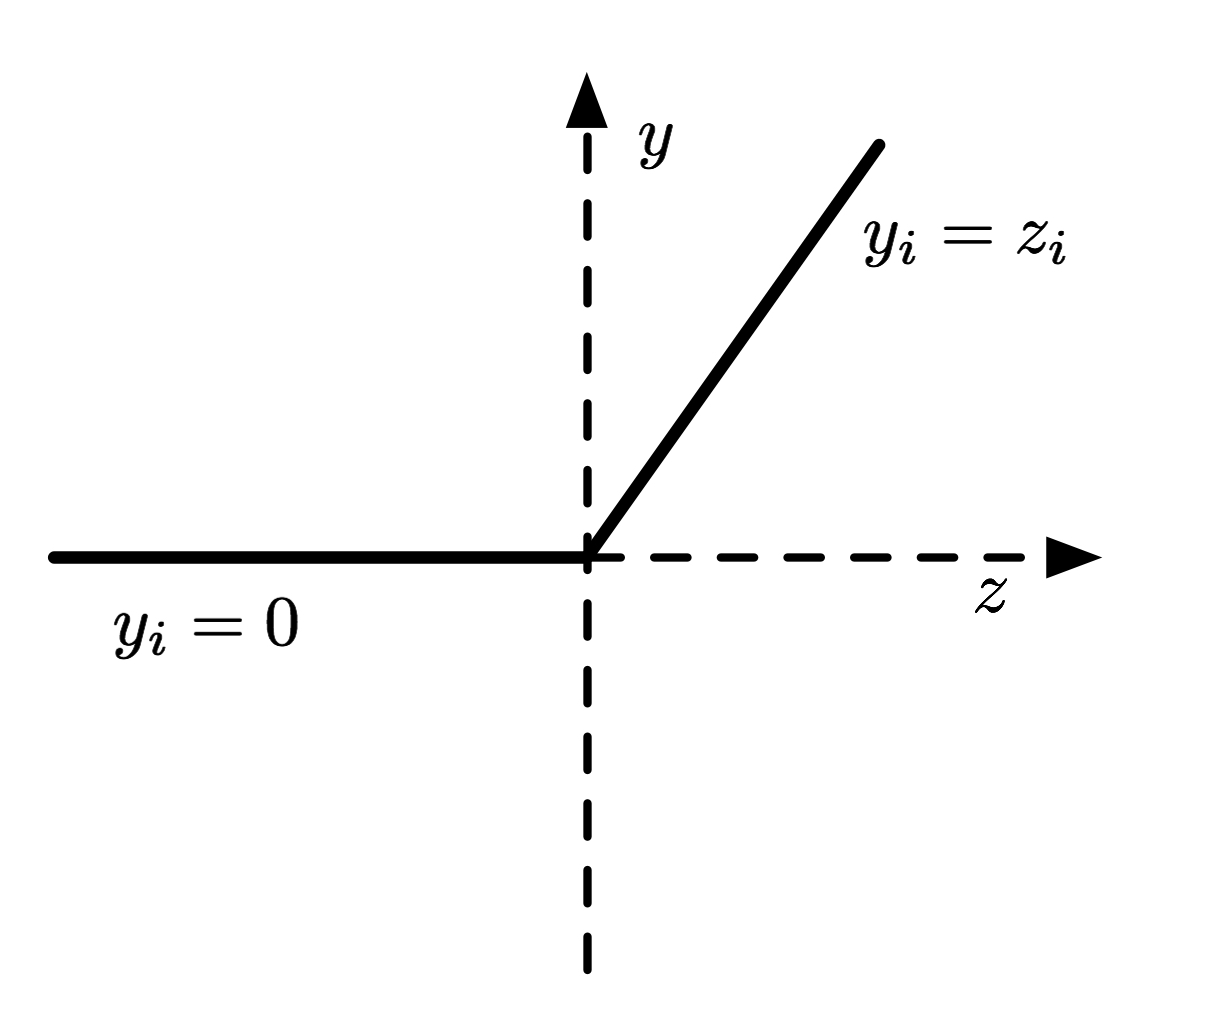
\includegraphics[height=30mm,width=\textwidth]{ch02_06_01.jpg}
			\caption{ReLU}
			\label{fig:ReLU}
		\end{subfigure}&
		\begin{subfigure}[c]{0.25\textwidth}
			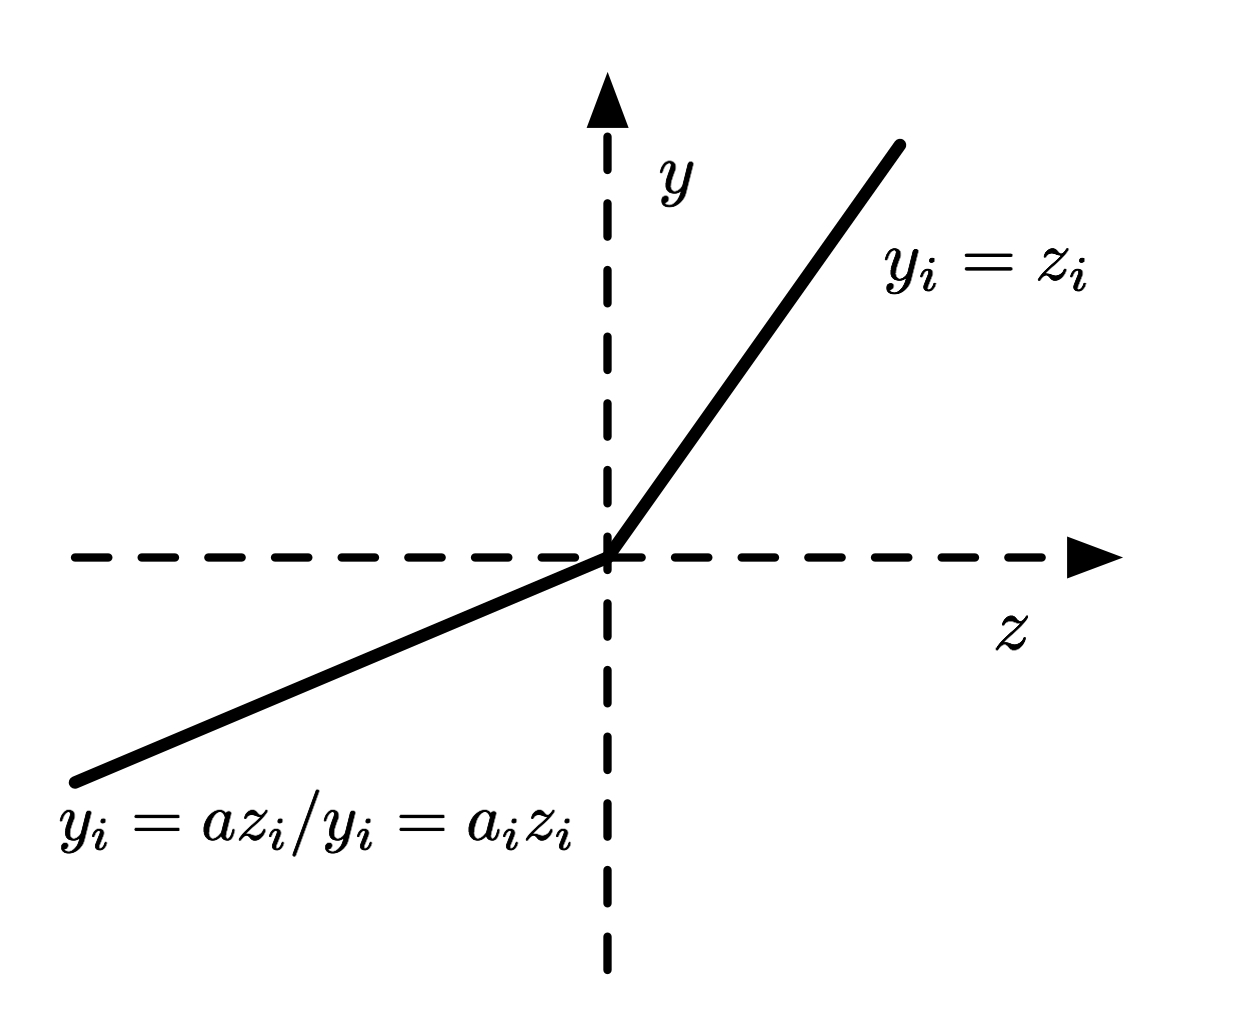
\includegraphics[height=30mm,width=\textwidth]{ch02_06_02.jpg}
			\caption{LReLU/PReLU}
			\label{fig:PReLU}
		\end{subfigure}\\
		\begin{subfigure}[c]{0.25\textwidth}
			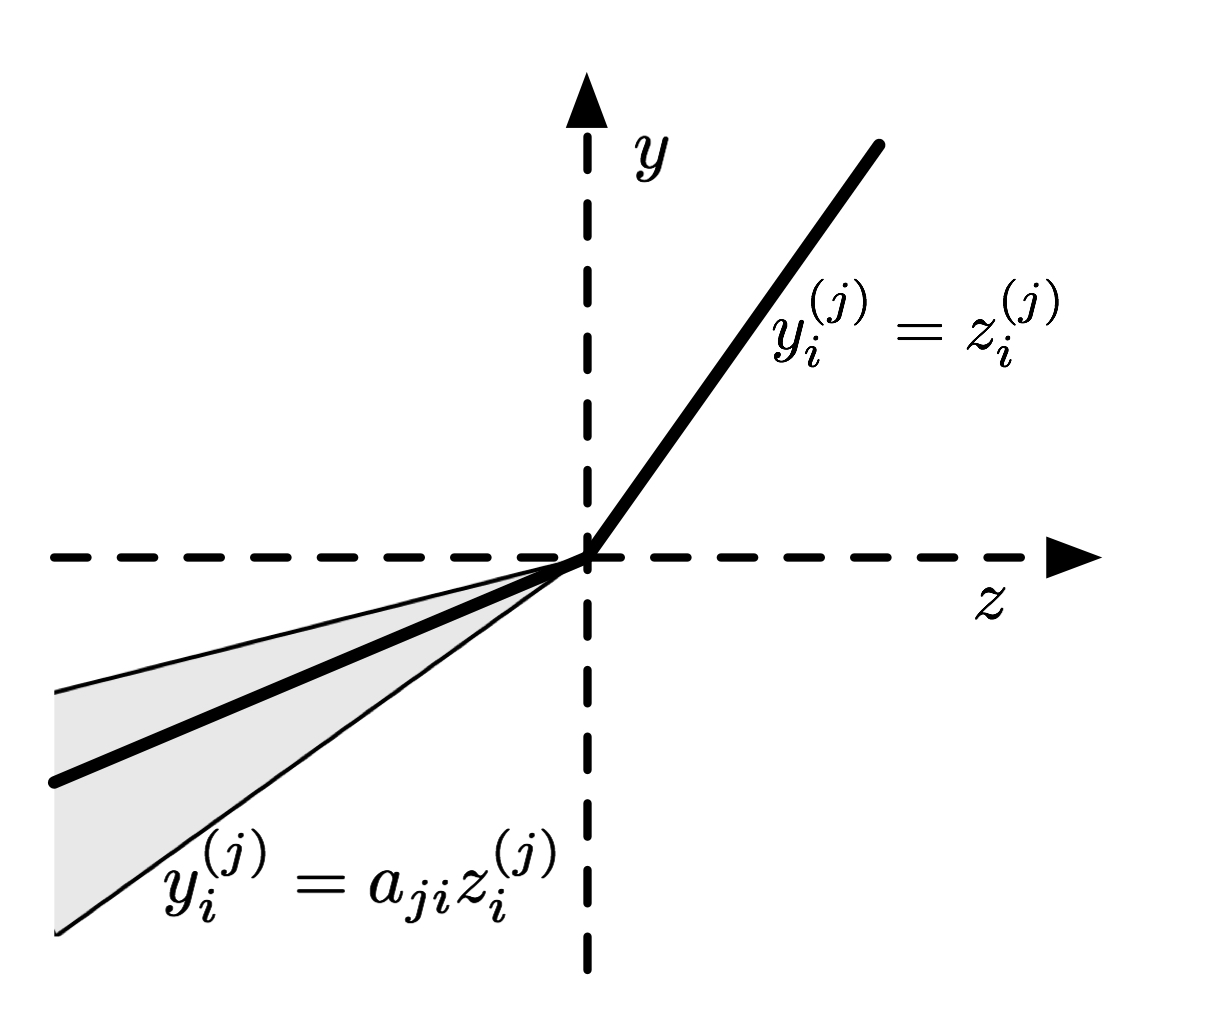
\includegraphics[height=30mm,width=\textwidth]{ch02_06_03.jpg}
			\caption{RReLU}
			\label{fig:RReLU}	
		\end{subfigure}&
		\begin{subfigure}[c]{0.25\textwidth}
			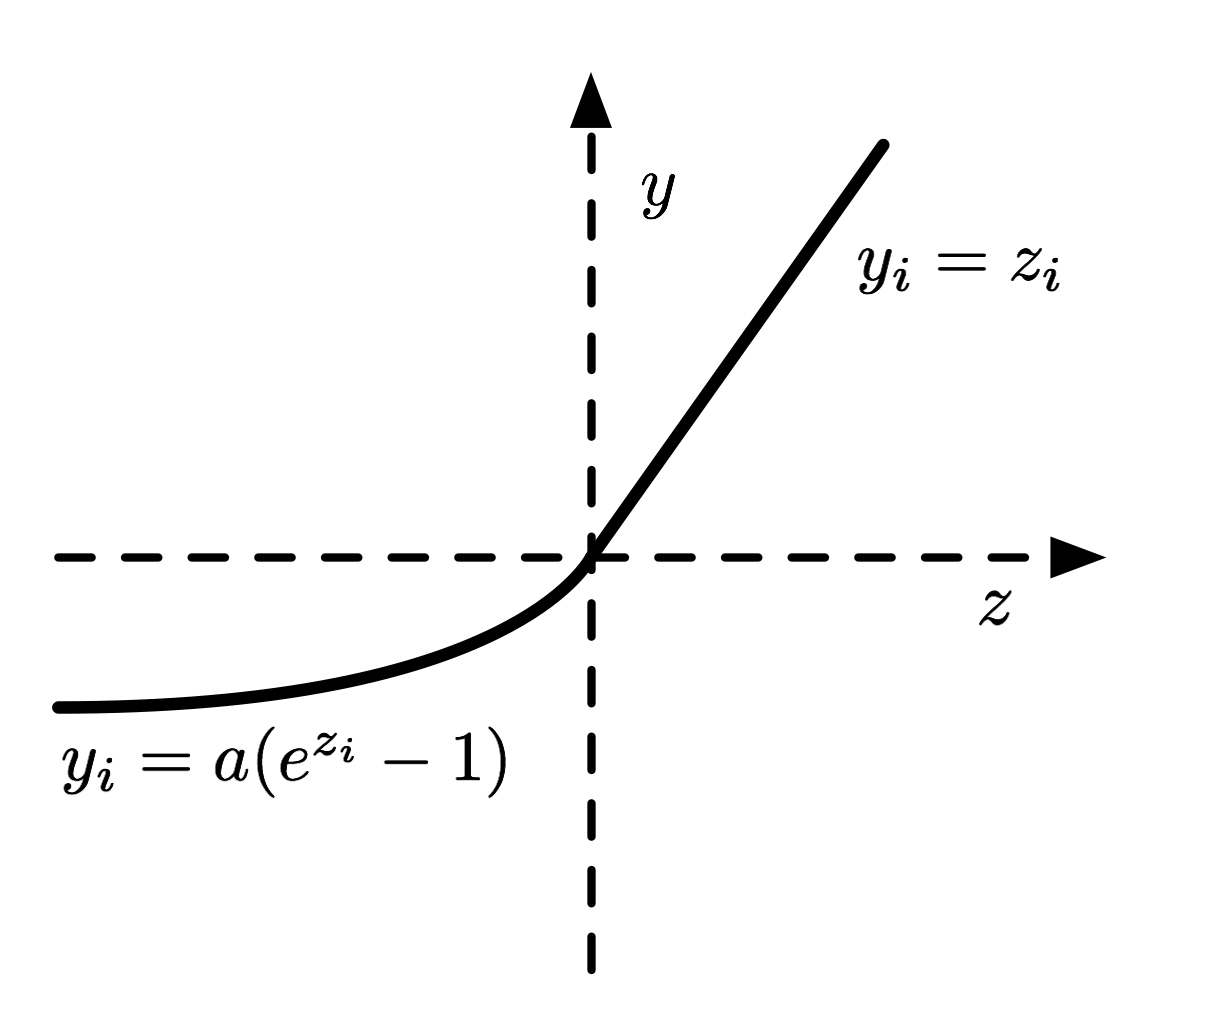
\includegraphics[height=30mm,width=\textwidth]{ch02_06_04.jpg}
			\caption{ELU}
			\label{fig:ELU}	
		\end{subfigure}				
	\end{tabular}    
	\caption[各种激活函数比较图]{ReLU,LReLU,PReLU,RRELU和ELU之间的比较,参数$\lambda $对于Leaky ReLU,是凭经验预定义的。对于PReLU是从训练数据中学习的。对于RReLU是一个随机变量,它是从训练中给定的均匀分布中抽取的,并在测试中保持固定。对于ELU是凭经验预定义的。}
	\label{fig:RRELU}
\end{figure}

\subsubsection{Maxout}
Maxout\cite{Goodfellow2014Generative}是一种替代性的非线性函数,能够近似任意连续函数,可以在每个空间位置获得跨多个通道的最大响应,函数定义如下:
$ a_{i,j,k}=\max_{k \in[1,K]}z_{i,j,k}$,其中$ z_{i,j,k} $是第$ i $通道的特征映射。由于ReLU实际上是maxout的一个特例,Maxout享有ReLU的所有好处,但参数会相应加倍。
\subsection{损失函数}
深度神经网络设计中的一个重要方面是损失函数的选择,损失函数是模型对数据拟合程度的反映,为特定任务选择合适的损失函数非常重要。我们在本小节中介绍三个有代表性的部分:softmax损失,铰链损失和对比损失。

\subsubsection{Softmax 损失}
Softmax损失结合softmax函数和交叉熵损失,是多项式逻辑损失和softmax的组合。给定训练$\{(x^{(i)}, y^{(i)}); i\in {1,\dots,N}, y^{(i)}\in {0,\dots,K-1}\}$,其中$ x ^ {(i)} $是$ i $ 输入图像区域,$ y^{(i)} $是它的类标签。第$ i $ 输入的第$ j $类的预测$ a_j ^ {(i)} $用以下softmax函数进行变换:
\begin{equation}
\label{eq:softmax}
p_j^{i} =e^{a_j^{(i)}}/{\sum_{l=0}^{K-1}e^{a_l^{(i)}}}
\end{equation}
Softmax将预测变成非负值,并将它们归一化以获得类别概率分布。这种概率预测用于计算多元逻辑损失,如下所示:

\begin{equation}
\label{eq:softmaxloss}
\begin{aligned}
\mathcal{L}_{softmax} =-\frac{1}{N}[\sum_{i=1}^{N}\sum_{j=0}^{K-1}1\{y^{(i)}=j\}\mathrm{log} p_j^{i}]
\end{aligned}
\end{equation}

\subsubsection{铰链损失}
铰链(Hinge)损失通常用于训练最大间隔的分类器,如支持向量机(Support Vector Machine,SVM)。多类SVM的铰链损失函数由公式(\ref{eq:L1_SVM_ml})定义,其中$ x_n $ 是给定的特征向量,而$ \ell_n \in [0,1,2,...,K-1] $指示$ K $类中的正确类标签。

\begin{equation} \label{eq:L1_SVM_ml}
\begin{aligned}
& \mathcal{L}_{Hinge} =\frac{1}{N}\sum_{n=1}^{N}\sum_{k=0}^{K-1}[\mathrm{max}(0,1-\delta(\ell_n,k)w^T x_n)]^p  \\
& \delta(\ell_n,k)=
\begin{cases}
1, & \text{if $\ell_n = k$} \\
-1, & \text{if $\ell_n \ne k$}
\end{cases}
\end{aligned}
\end{equation}

注意如果$ p = 1 $,公式(\ref{eq:L1_SVM_ml})是$ L_1 $损失,而如果$ p = 2 $,则是平方铰链损失$ L_2$。

\subsubsection{对比损失}
对比(Contrastive)损失\cite{Shaham2017Learning}常用于训练孪生多通路网络,属于弱监督方法,用于从标记为匹配或不匹配的数据实例对中学习相似性度量。 给定第$i$对数据$(x_{\alpha} ^{(i)},x_{\beta} ^{(i)})$,令$(z_{\alpha} ^{(i,l)},z_{\beta} ^{(i,l)})$表示其对应的第$l$个($l \in [1,\dots,L]$)层的输出对。图像对通过两个相同的CNN分别传递,并将最终图层的特征向量送入到损失函数,对比损失$ \mathcal {L} _l $被定义为:

\begin{equation}
\begin{aligned}
\label{ContrastiveLoss}
 \mathcal{L}_{contrastive}= \frac{1}{2N}\sum_{n=1}^{N}\sum_{l=1}^{L}(y)d^{(i,L)} + (1-y)\max(\mathrm{m}-d^{(i,L)}, 0) 
\end{aligned}
\end{equation}
其中$d^{(i,L)} = ||z_{\alpha}^{(i,l)} - z_{\beta}^{(i,l)}||_2^2$,是$ z ^{(i,l)}_\alpha $和$ z^{(i,l)}_\beta $之间的相似度,$ m $是影响非匹配对的边界参数。如果$(x_{\alpha} ^{(i)},x_{\beta} ^{(i)})$是匹配的对,那么$ y = 1 $。否则,$ y = 0 $。这种损失函数也被称为单边界参数损失函数。Lin等\cite{Zhu2016b}利用这种单边界损失函数在所有对上对网络进行训练时,会导致检索结果急剧下降。同时,仅在非匹配对上进行内部调整时,性能得到更好的保留。 这表明处理丢失函数中的匹配对是造成丢失的原因。 虽然非匹配对的召回率是稳定的,但处理匹配对是召回率下降的主要原因。 为了解决这个问题提出了一个双边界损失函数,它为匹配对添加了另一个边界参数。定义为:

\begin{equation}
\label{DMContrastiveLoss}
\mathcal{L}_{doublecontrastive}= \frac{1}{2N}\sum_{n=1}^{N}\sum_{l=1}^{L}(y)\max(d^{(i,L)}-\mathrm{m}_1,0) + (1-y)\max(\mathrm{m}_2-d^{(i,L)}, 0)
\end{equation}
\subsection{优化方法}
在本小节中,我们将讨论优化CNN训练的一些关键技术。

\subsubsection{权重初始化}
通常深度CNN模型具有大量的参数并且损失函数是非凸的,导致难以训练。为了实现训练中的快速收敛,正确的初始化是最重要的先决条件之一。偏置参数可以初始化为零,而权重参数的设置需打破同一层隐藏单元之间的对称性。例如,如果我们简单地将所有权重初始化为相同的值,例如0或1,那么同一层的每个隐藏单元将得到完全相同的信号。
有些启发式方法可用于选择权重的初始大小,最常用的初始化方法是根据高斯或均匀分布随机设置权重。Glorot和Bengio\cite{Glorot2010}提出初始化$m$个输入$n$个输出可根据零均值和特定方差的分布设置权重:$ Var(W_{i,j})~ \sqrt{6} / \sqrt{m + n} $,也被称为“Xavier”。但是初始化时强加的性质可能在学习开始进行后不能保持;可能成功提高了优化速度,但意外地增大了泛化误差,这些初始化方法往往不会带来最佳效果。在实践中,我们通常需要将权重范围视为超参数进行调参估计。

\subsubsection{随机梯度下降}\label{SGD_optimization}
一般使用批梯度下降(stochastic gradient descent,SGD)来更新模型参数,采用反向传播算法计算损失函数的梯度。梯度下降算法将目标$ J(\theta)$的参数$ \theta $更新为$ \theta_{t + 1} = \theta_t - \alpha \nabla_\theta E [J(\theta_t)] $,其中$ E [J(\theta_t)] $是整个训练集上$ J(\theta)$的期望值,$ \alpha $是学习率。随机梯度下降根据单个随机选取的示例$(x ^ {(t)},y ^ {(t)})$进行梯度更新:
\begin{equation}
\label{eq:SGD}
\theta_{t+1} = \theta_t - \mu_t \nabla_\theta J(\theta_t; x^{(t)},y^{(t)})
\end{equation}

实际上,SGD中的每个参数更新都是针对小批量数据(mini-batch)而不是单个示例,这可以帮助减少参数更新中的变化并且可以导致更稳定的收敛性。收敛速度由学习率$ \mu_t $控制。在面对小而连续的梯度但是含有很多噪声的时候,带动量(Momentum)SGD算法可以很好的加速学习为了加速训练使当前更新梯度取决于历史梯度在相关方向上累积速度向量信息,经典的带动量SGD更新由下式给出:
\begin{equation}    \label{eq:mSGD}
\begin{aligned}
   & v_{t+1} = \theta_t - \mu_t \nabla_\theta J(\theta_t; x^{(t)},y^{(t)})\\
   & \theta_{t+1} = \theta_t +v_{t+1} 
\end{aligned}
\end{equation}
其中$v_{t+1}$是当前速度矢量,是通常设置动量衰减参数$\mu$为0.9。 在梯度下降优化中使用动量的另一种方式Nesterov\cite{Krizhevsky2012}:
\begin{equation}
    \label{eq:nSGD}
    v_{t+1} = \gamma v_t - \mu_t \nabla_\theta J(\theta_t; x^{(t)},y^{(t)})
\end{equation}
\ref{eq:nSGD}首先计算当前梯度,然后沿更新的累积梯度方向移动,与经典动量\ref{eq:mSGD}相比,Nesterov首先沿先前累积梯度的方向移动vt,计算梯度,然后进行梯度更新。这种预期的更新可以防止优化移动太快,并获得更好的性能。一种常用的方法是使用小的恒定学习速率,在初始阶段给出稳定的收敛,然后随着收敛速度的减慢而降低学习速率。除了这种人工手动设置学习率的方法之外,还有很多自适应学习率的方法,如Adam\cite{Kingma2014Adam}利用梯度的一阶矩估计和二阶矩估计动态调整每个参数的学习率。此外,并行化的SGD方法能够提高SGD以适合并行的大规模机器学习。

\subsubsection{批量归一化}
批量归一化(Batch Normalization)\cite{Ioffe2014Batch}的提出旨在加速深度神经网络的整个训练过程。他们认为内部协变量偏移,即深度网络内部节点分布的变化将会减慢网络训练的速度。为此提出了一种称为批量归一化的有效方法来部分缓解这种现象。它通过归一化数据使其服从标准高斯分布来修复了各层输入的方式和差异。批量归一化可以理解为在网络的每一层之前都做预处理,只是这种操作以另一种方式与网络集成在了一起。除了加速训练外,批量归一化还使我们能够使用更高的学习速率而不存在发散风险,并且可以通过防止网络陷入饱和模式来使用饱和非线性。
\subsection{正则化方法}
过拟合在深层CNN中是一个不容忽视的问题,可以通过正则化来有效降低过度拟合问题。在下面的小节中,我们介绍一些有效的正则化技术。
\subsubsection{$p$范数正则化}
正则化通过增加惩罚模型复杂性的额外项来修改目标函数,若损失函数为$L(\theta; x; y)$,则正则化损失将为:
\begin{equation}
E(\theta ; x; y)= L(\theta ; x; y)+\lambda R(\theta ) 
\end{equation}
其中$R(\theta)$是正则化项,并且$\lambda$是正则化项参数。
$p$-范数正则化函数通常用作$R(\theta)=\sum_j||\theta_j||_p^p$,当$p=1$,$p$-范数是凸的,这使得目标函数更容易优化,并使这个函数具有稀疏性,使得参数变小倾向接近零。对于$p = 2$,“2-范数正则化”通常称为“权重衰减”,使得参数更平均; 当$p<1$时,$p$-范数正则化更多地利用了权重的稀疏效应,但却导致了非凸函数。
\subsubsection{随机失活}
\label{Section Dropout}
随机失活(Dropout)\cite{Srivastava2014a} 提供了一大类模型的正则化方法,其可以被认为是集成大量深层神经网络的实用Bagging方法,能够训练和评估指数级数量的神经网络,计算方便但功能强大。在训练的时候,随机失活的实现方法是让神经元以超参数$p$的概率被激活或者被设置为0。在训练过程中,随机失活可以被认为是对完整的神经网络抽样出一些子集,每次基于输入数据只更新子网络的参数(然而,数量巨大的子网络们并不是相互独立的,因为它们都共享参数)。在测试过程中不使用随机失活,可以理解为是对数量巨大的子网络们做了模型集成,以此来计算出一个平均的预测。

研究指出在使用费舍尔信息矩阵(fisher information matrix)的对角逆矩阵的期望对特征进行数值范围调整后,再进行L2正则化这一操作,与随机失活正则化是一阶等价的。而DropConnect\cite{Wan2013Regularization}将Dropout的思想更进一步改进,DropConnect不是将神经元的输出设置为零,而是以概率$ p $选择完全连接层的权重$ W $设置为零。\figurename {\ref{fig:CNN_DropConnect}}说明了无Dropout,Dropout和DropConnect网络之间的差异。

\begin{figure}
	\centering
	\begin{tabular}[c]{ccc}
		\begin{subfigure}[c]{0.27\textwidth}
			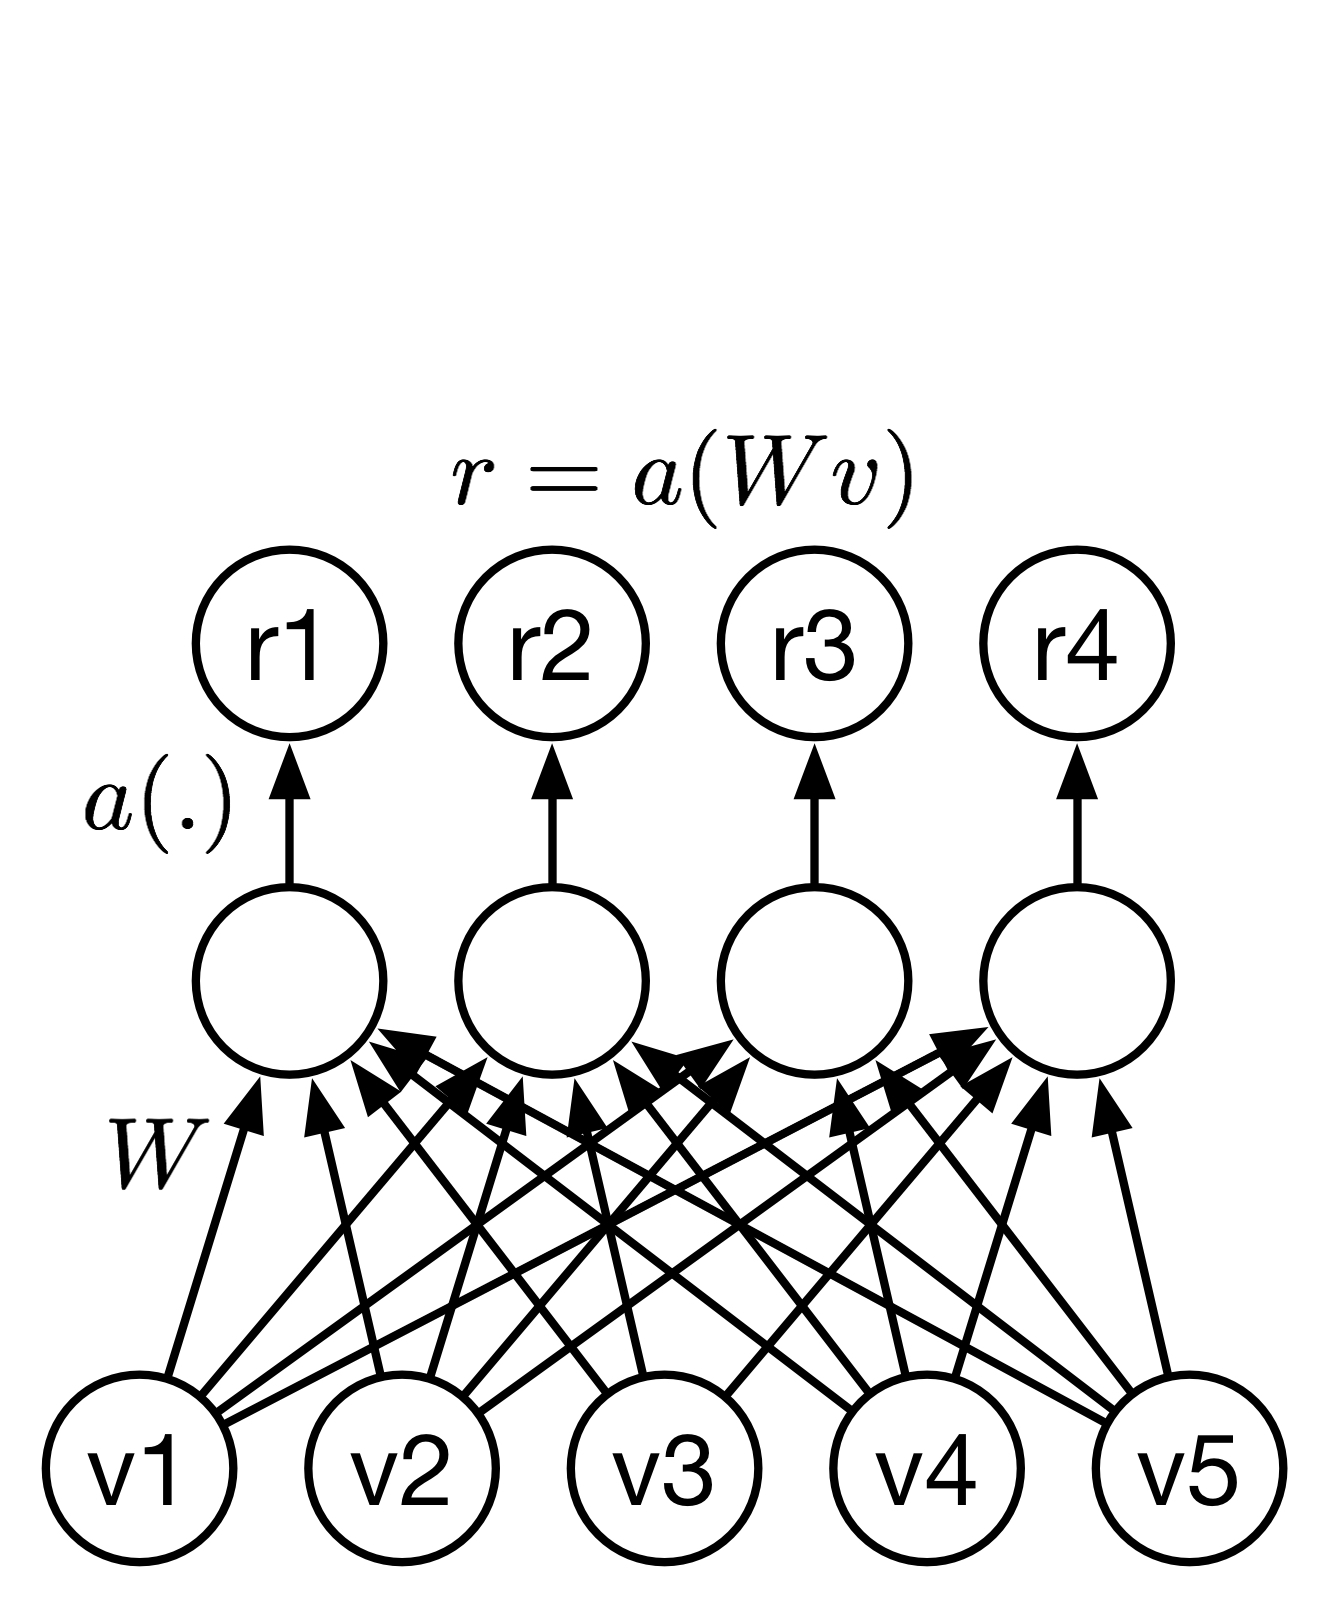
\includegraphics[width=\textwidth]{ch02_07_01.jpg}
			\caption{No-Drop}
			\label{fig:nodrop}
		\end{subfigure}&
		\begin{subfigure}[c]{0.27\textwidth}
			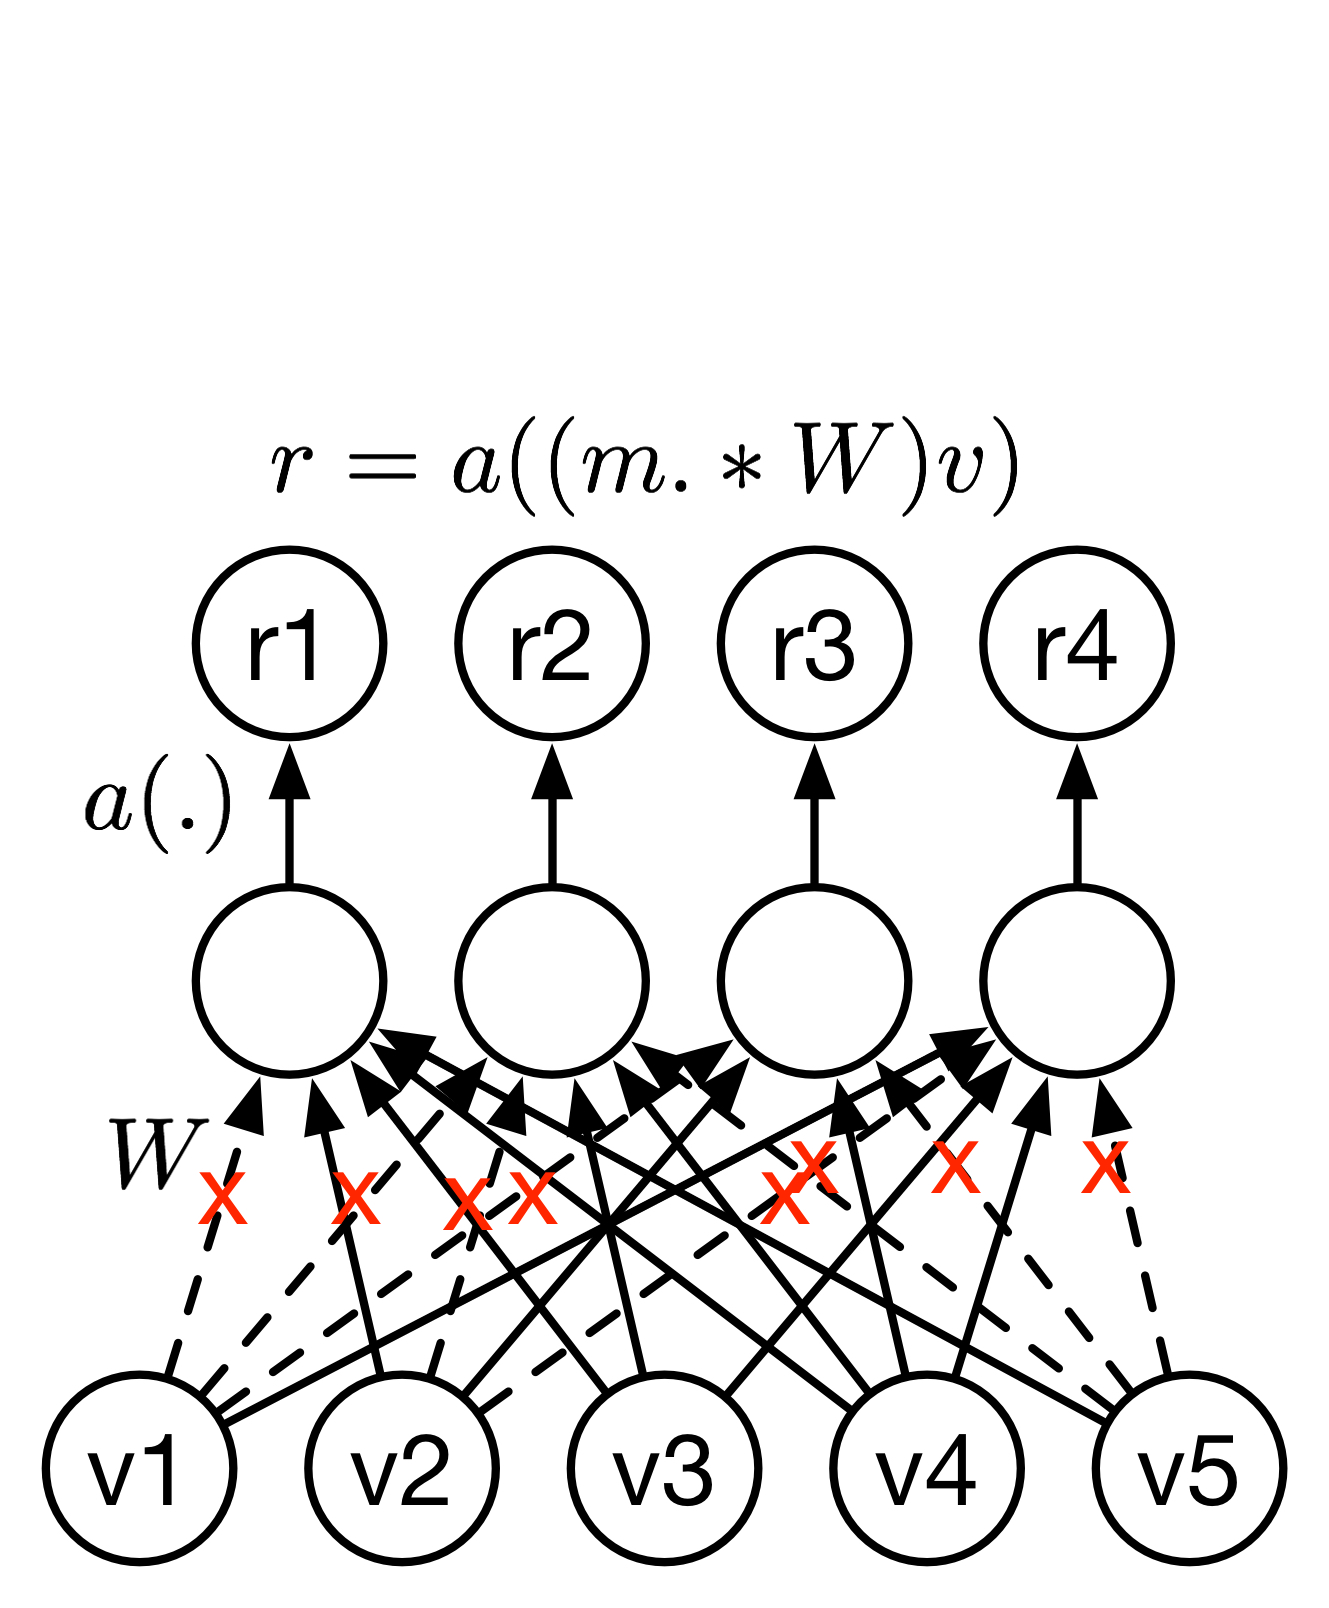
\includegraphics[width=\textwidth]{ch02_07_02.jpg}
			\caption{DropOut}
			\label{fig:dropout}
		\end{subfigure}&
		\begin{subfigure}[c]{0.27\textwidth}
			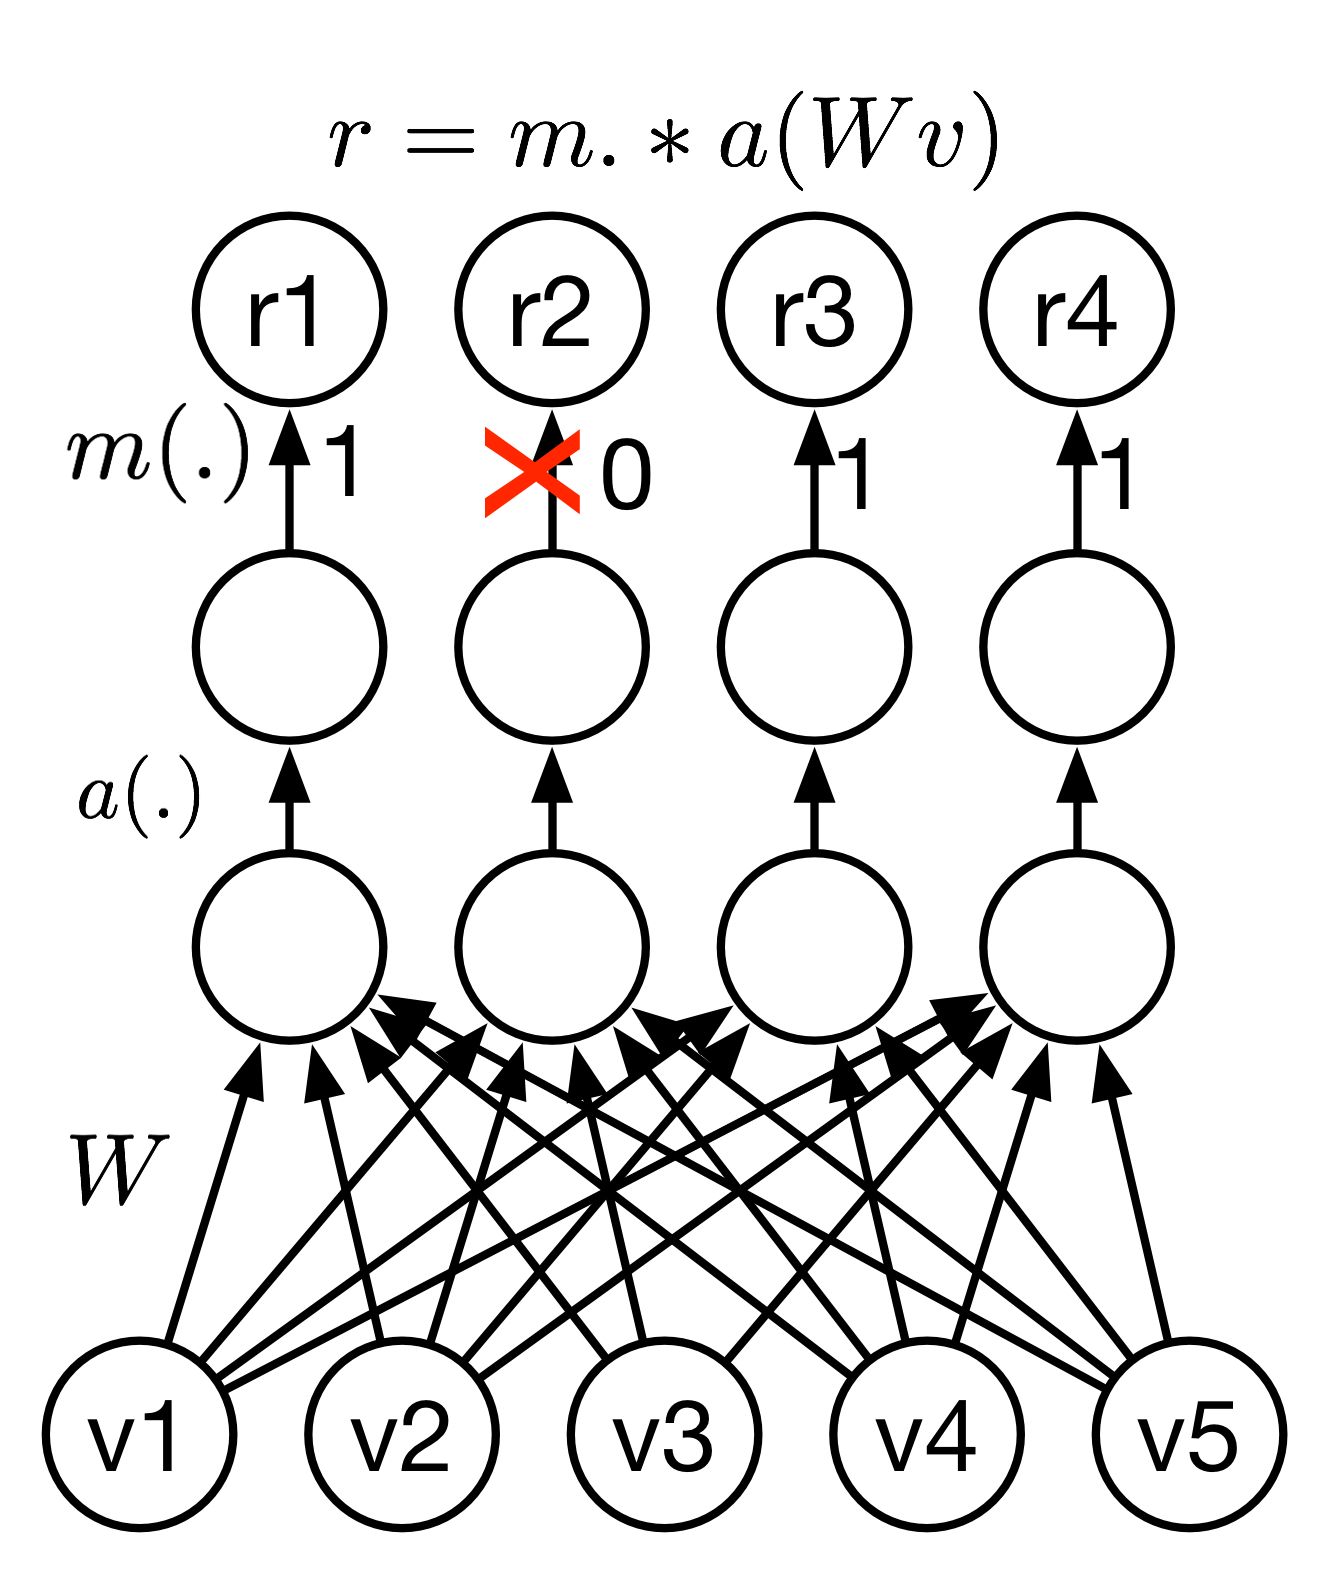
\includegraphics[width=\textwidth]{ch02_07_03.jpg}
			\caption{DropConnect}
			\label{fig:dropconnect}	
		\end{subfigure}			
	\end{tabular}    
	\caption{无Dropout网络,DropOut网络和DropConnect网络的图示。}
	\label{fig:CNN_DropConnect}
\end{figure}

\section{小结与讨论}

本章首先对学习算法和神经网络基本方法进行了梳理,包括卷积神经网络和深度卷积神经网络模型进行了分析,进一步对无监督深度学习进行了概述。同时对深度学习应用于医学图像中涉及的分类、检测和分割应用算法从原理上进行了分析。最后对深度学习中相关核心技术了描述,涉及激活函数、损失函数、优化方法和正则化。 